\documentclass[a4paper,adobefonts,11pt,UTF8]{book}

%type chinese characters
\usepackage{ctex}

%Bibliography
\usepackage{chapterbib}
\usepackage[sectionbib,square,super,sort&compress]{natbib}


%generate index of book
\usepackage{makeidx}

\graphicspath{{../img/}}

%modify the headheight at least 13.5pt
\usepackage[headheight=13.6pt]{geometry}

%
\usepackage{fontspec}

%unicode
\usepackage{xunicode}

%
\usepackage{xltxtra}

%mathematics package
\usepackage{amsmath}

%mathematics symbols
\usepackage{amssymb}

%origin print package
\usepackage{verbatim}

%draw graphics use tikz and so on.
\usepackage{graphicx}

%set graphics path which used in the book.
\graphicspath{{../img/}}

%colorful table
\usepackage{colortbl}

%set color use origin name directly.
\usepackage[svgnames,table]{xcolor}

%
\usepackage[figuresright]{rotating}

% generate longtable which could across pages.
\usepackage{longtable}

%
\usepackage{multirow}

%
\usepackage{adjustbox}


%
\newcommand\mgape[1]{\gape{$\vcenter{\hbox{#1}}$}}

%
\usepackage{array}

%
\usepackage{makecell}

%
\usepackage{ulem}

%
\usepackage{color}

% draw graphics use tikz package
\usepackage{tikz}

%
\usepackage{listings}
\lstset{
  basicstyle=\ttfamily,
  showstringspaces=false,
  commentstyle=\color{red},
  keywordstyle=\color{blue},
  columns=flexible,
  backgroundcolor=\color{lightgray},
  extendedchars=true,
  basicstyle=\footnotesize\ttfamily,
  showstringspaces=false,
  showspaces=false,
  numbers=left,
  numberstyle=\footnotesize,
  numbersep=9pt,
  tabsize=2,
  breaklines=true,
  showtabs=false,
  captionpos=b
}

%
\usepackage{bashful}

%set book information including bookmarksnumbered,pdfencoding,
%pdfauthor,pdfpagelayout,breaklinks,colorlinks,linkcolor,
%urlcolor,and so on.
\usepackage[bookmarksnumbered,pdfencoding=auto,pdfauthor={穷屌丝联盟},pdfpagelayout=TwoPageRight,breaklinks,colorlinks,linkcolor=RoyalBlue,urlcolor=blue,colorlinks=true]{hyperref}

%add more list types.
\usepackage{paralist}

%set page styles
\usepackage{fancyhdr}

\pagestyle{fancy}
\fancyhf{}
\fancyhead[LE,RO]{\thepage}
\fancyhead[RE]{\leftmark}
\fancyhead[RO]{\rightmark}
\fancypagestyle{plain}{
  \fancyhf{}
  \renewcommand{\headrulewidth}{0pt}
}


%titlepage \titleGM
\newcommand*{\plogo}{\fbox{$\mathcal{PL}$}} % Generic publisher logo
%--------------------------------------------------------------------
% TITLE PAGE
%--------------------------------------------------------------------

\newcommand*{\titleGM}{\begingroup % Create the command for including the title page in the document
\hbox{ % Horizontal box
\hspace*{0.2\textwidth} % Whitespace to the left of the title page
\rule{1pt}{\textheight} % Vertical line
\hspace*{0.05\textwidth} % Whitespace between the vertical line and title page text
\parbox[b]{0.75\textwidth}{ % Paragraph box which restricts text to less than the width of the page
{\noindent\Huge\bfseries Notes Collection of \\[0.5\baselineskip] General Knowledge}\\[2\baselineskip] % Title
{\large \textit{General Knowledge}}\\[4\baselineskip] % Tagline or further description
{\Large \textsc{theqiong.com}} % Author name

\vspace{0.5\textheight} % Whitespace between the title block and the publisher
{\noindent 穷屌丝联盟}\\[\baselineskip] % Publisher and logo
}}
\endgroup}
%


%lstlisting[language=JavsScript]
% Taken from Lena Herrmann at 
% http://lenaherrmann.net/2010/05/20/javascript-syntax-highlighting-in-the-latex-listings-package
\definecolor{lightgray}{rgb}{.9,.9,.9}
\definecolor{darkgray}{rgb}{.4,.4,.4}
\definecolor{purple}{rgb}{0.65,0.12,0.82}

%lstlisting package -----------
% JavaScript
%------------------------------
\lstdefinelanguage{JavaScript}
{
  keywords={typeof,new,ture,false,catch,function,return,null,switch,var,if,in,while,do,else,case,break},
  keywordstyle=\color{blue}\bfseries,
  ndkeywords={class,export,boolean,throw,implements,import,this},
  ndkeywordstyle=\color{darkgray}\bfseries,
  identifierstyle=\color{black},
  sensitive=false,
  comment=[l]{//},
  morecomments[s]{/*}{*/},
  commentstyle=\color{purple}\ttfamily,
  stringstyle=\color{red}\ttfamily,
  morestring=[b]',
  morestring=[b]"
}

\lstdefinelanguage{Scheme}
{morekeywords={,lambda, cond, case, display, let, import, quote, quasiquote, unquote,
define, begin, newline, if, list, apply, null?, car, cdr, or, not, and, for-each, 
make-vector, vector-length, vector-ref, vector-set!, eqv?, eq?, equal?, else, set!, 
define-record-type, fields, mutable, immutable, assert, parent, with-exception-handler, }
sensitive=false,
morecomment=[l]{;},
morecomment=[s]{/*}{*/},
morestring=[b]",
}

\lstdefinelanguage{CSS}{
  morekeywords={accelerator,azimuth,background,background-attachment,
    background-color,background-image,background-position,
    background-position-x,background-position-y,background-repeat,
    behavior,border,border-bottom,border-bottom-color,
    border-bottom-style,border-bottom-width,border-collapse,
    border-color,border-left,border-left-color,border-left-style,
    border-left-width,border-right,border-right-color,
    border-right-style,border-right-width,border-spacing,
    border-style,border-top,border-top-color,border-top-style,
    border-top-width,border-width,bottom,caption-side,clear,
    clip,color,content,counter-increment,counter-reset,cue,
    cue-after,cue-before,cursor,direction,display,elevation,
    empty-cells,filter,float,font,font-family,font-size,
    font-size-adjust,font-stretch,font-style,font-variant,
    font-weight,height,ime-mode,include-source,
    layer-background-color,layer-background-image,layout-flow,
    layout-grid,layout-grid-char,layout-grid-char-spacing,
    layout-grid-line,layout-grid-mode,layout-grid-type,left,
    letter-spacing,line-break,line-height,list-style,
    list-style-image,list-style-position,list-style-type,margin,
    margin-bottom,margin-left,margin-right,margin-top,
    marker-offset,marks,max-height,max-width,min-height,
    min-width,-moz-binding,-moz-border-radius,
    -moz-border-radius-topleft,-moz-border-radius-topright,
    -moz-border-radius-bottomright,-moz-border-radius-bottomleft,
    -moz-border-top-colors,-moz-border-right-colors,
    -moz-border-bottom-colors,-moz-border-left-colors,-moz-opacity,
    -moz-outline,-moz-outline-color,-moz-outline-style,
    -moz-outline-width,-moz-user-focus,-moz-user-input,
    -moz-user-modify,-moz-user-select,orphans,outline,
    outline-color,outline-style,outline-width,overflow,
    overflow-X,overflow-Y,padding,padding-bottom,padding-left,
    padding-right,padding-top,page,page-break-after,
    page-break-before,page-break-inside,pause,pause-after,
    pause-before,pitch,pitch-range,play-during,position,quotes,
    -replace,richness,right,ruby-align,ruby-overhang,
    ruby-position,-set-link-source,size,speak,speak-header,
    speak-numeral,speak-punctuation,speech-rate,stress,
    scrollbar-arrow-color,scrollbar-base-color,
    scrollbar-dark-shadow-color,scrollbar-face-color,
    scrollbar-highlight-color,scrollbar-shadow-color,
    scrollbar-3d-light-color,scrollbar-track-color,table-layout,
    text-align,text-align-last,text-decoration,text-indent,
    text-justify,text-overflow,text-shadow,text-transform,
    text-autospace,text-kashida-space,text-underline-position,top,
    unicode-bidi,-use-link-source,vertical-align,visibility,
    voice-family,volume,white-space,widows,width,word-break,
    word-spacing,word-wrap,writing-mode,z-index,zoom},
  morestring=[s]{:}{;},
  sensitive,
  morecomment=[s]{/*}{*/}
}


\renewcommand{\chaptername}{}
%%\titleformat{\chapter}[block]{\center\Huge}{\chaptername}{20pt}{}
%%\titleformat{\chapter}[block]{\center\Huge}{\chaptername}{20pt}{}
%%\makeatletter
\renewcommand{\bibname}{来源}



\setmainfont[Mapping=tex-text]{Minion Pro}

\makeindex


\title{{\zihao{1}General Knowledge}}
\author{{\zihao{3}穷屌丝联盟}}
\date{\today}








\begin{document}

\begin{titlepage}
\addcontentsline{toc}{chapter}{Cover}

\pagestyle{empty} % Removes page numbers

\titleGM % This command includes the title page


\end{titlepage}

\maketitle
\tableofcontents
\listoffigures
\listoftables
\printindex

\chapter{记录今天就是记录历史}


\begin{center} 陈~虻\cite{chengmeng_immortal} \end{center}

出处:网络

一个著名的学者曾经说过:历史都是当代史。

从这个意义上来说,记录过去就是记录今天,而今天又是明天的历史,记录今天也就是在记录历史。若干年之后,当我们的后人向我们问起今天的历史时,我们给他们展示的应该是那些有价值、永远不会沉沦的东西,而这些也恰恰是纪录片工作者所应该具有的历史使命感。

那么,对于电视纪录片工作者来说,我们应该怎样记录今天的历史,应该带着一种什么样的心态去记录历史?这是值得我们共同探讨的问题。

以各种人物、各种角度为切入口,记录历史。

在我们以往宣传的人物形象中,小人物、或者普通人的形象占了很小的篇幅,可以说,在当代中国的媒体上,我们并没有由小人物构成的一系列形象,也没有一部完全由小人物构成的历史。

自从《东方时空》以一个栏目、每天一期的播出量开始“讲述老姓自己的故事”以来,从小人物为切入点来记录历史,以小人物来展示中国历史这段流程的工作已经在开始进行了。它除了转变了人们长期以来形成的一种意识之外,还为中国的纪录片作了一些努力。

以前,我们的拍摄对象都是出于一种被拍摄状态,在《生活空间》的节目里,被拍摄对象则处于一种生活状态,这就改变了人们长期以来习惯的一种视觉符号,丰富了他们的视听语汇,同时还教化和培养了一批观众,使他们可以读懂这些语汇,这是用普通人作为突破口来完成的一种教化,一种意识的转变。这种转变之后,一旦人们能够接受真实,读懂真实和识别真实之后,其实更需要用真实的光芒去照亮的领域远比这个更多。因此,从“讲述老百姓自己的故事”开始,我们从普通人的切入口进入纪录片的创作,我们提出:为未来留下一部由小人物构成的历史。然而,对中国的纪录片来说,仅仅局限于小人物是远远不够的,为未来留下一部由小人物构成的历史是必须的,但纪录片决不等于只能由小人物来留历史,还应该从大人物,或者古人,或者是未来的人,各种的角度切进去,只有这样记录的历史才是真正的历史。

\section{纪录片应与其他的艺术门类相通}

%%\textbf{纪录片应与其他的艺术门类相通}

首先,纪录片是一种艺术品,它仅仅是在电视圈内被认知是不够的,纪录片老是由搞片子的人来研究也是不够的,纪录片应该和其他的艺术门类相通。

如果都是做纪录片的来研究纪录片,我们所研究的只能是技术;而如果让一个文学批语家来研究纪录片,他就不会去研究镜头,不会去研究剪接,他会说主题,说节目所包含的内容。因此如果对纪录片的研究仅限于一个窄小的圈子,那么大家也只能去研究技术,因为当你进入一个专业的时候,实际上也就进入了一个狭小的空间。对中国今天的纪录片来说,我们现在需要的是一桶水的来源,就需要打破狭小的专业,需要研究另外的领域,虽然他们也许只是一勺水,但把这一勺水都端过来就给了我们一桶水。

其次,纪录片不应该成为很孤立的、很专业的东西,它应该和社会发生多方面的联系,它最终的结果还是要和这个时代的敏感神经发生联系,和这个时代的重大问题发生联系。如果没有这种联系,就不可能和观众找到联系。举一个极端的例子:如果一个很有意思的历史事件突出发生,有人用非常差的技术,非常业余的水平去把它记录下来,只要记录得完整了,它就可能成为一部经典的纪录片。在这个极端的例子里,历史是非常重要的东西,技术的东西可以消失,因为在这里最中心的东西凸显出来了,这也是最核心的东西。又一个比喻,用来比喻中国纪录片的局部是恰当的:卢浮宫里挂的都是油画,而我们现在都是画素描的,每一位画油画的大师都是从素描开始的,但不是所有画素描的人都可以把油画挂在这里。我们现在整个纪录片的发展状况都是在解决问题,我们群体的状况是还没有解决技术问题,我们缺乏合格的人才。因此,我们应该知道自己的状况,踏踏实实地从一点一滴入手。但是我们肩负着双重责任,一方面是自己的业务需要不断提高,另一方面,这段历史谁来记录?油画的时代,你不能还是画素描,你也得凑凑合合地画油画。

\section{纪录片面临的挑战:对社会关注能力的挑战}

我们和国际纪录片的差距在哪?第一,技术上的差距。比如录音质量和画面影像质量,技术差距中最明显的是声音的差距。第二,艺术上的差距。国外的纪录片大师不单单是做纪录片的,他首先是一个艺术家,他具有一定的艺术修养,对生活的认识以及了解的程度已经达到了一定的水准,因为只有达到了这一水平之后,他才能把自己对生活的理解通过视觉的手段表现出来,这种修养是一种国民素质,需要一种环境,需要一代人一代人积累。而这一点恰恰是我们所欠缺的。

这里有必要谈一下纪录片与故事片的不同收视心理。纪录片最重要的是唤起我们的理性到场,它不是诉诸于人们的非理性,不是让你进入一种很本能的感官享受,相反,它是呼唤你的理性到场,让你去思考这个问题,进入这个问题的核心,因为这些问题就发生在你的身边,发生在你所生活的城市,所以你无法逃避,你必须面对。当你欣赏一部纪录片时,实际上也是和创作者的一种心灵的对话,在这个过程中,你必须要求自己的理性时时刻刻处于十分清醒的状态,这也是纪录片与故事片在观看心理上最本质的不同之处。故事片是靠怀节、从感情上来打动人,靠感官来席卷观众;纪录片除了在情节和情感上打动人之外,还要求观众用另外的东西来参与,这就是清醒的理性精神。

因此,中国纪录片面临的挑战,不光是技术上的挑战,还包括创作者对社会关注能力的挑战,即我们选择什么、关注什么。

中国的纪录片创作者必须回到我们的日常生活、我们现实的土地上来,关注中国现实生活中所出现的种种问题,这可以说是中国纪录片生命和基础。

现在我们有很多纪录片热衷于讲述一个悲欢离合的故事,如果仅仅是这样一个故事,而没有和大的文化背景、时代背景、民族命运相关联的话,其实是背离了纪录片的本原。因为故事片更好看,更能使人动情。现在我们需要解决的一个问题就是:因为我们走得太远,以至于忘了我们为什么要出发。当我们认真地去研究怎样去拍纪录片的时候,或许我们已经淡忘了我们为什么要拍纪录片。也就是说,当你过于进入、过于热衷于一个东西时,你就需要放弃这个东西。你只有出去了才能进来,也只有进来了才能出去。现在中国的纪录片恰恰需要跳出去。不要过于陷入,你才能反过来冷静地加以审视;如果一个人过于热爱,这东西就已经不再是它本身,已经变成了你的一种热爱,强加了你许多个人的东西,而不识事件本身。“太极”里说,练太极的人中太想练成的和三心二意地人都练不成。你必须保持一定状态,得到一种真传。按照西方的美学表述就是,距离产生美,必须有一定的距离,贴得太近反而什么也看不见。

\section{关于纪实的问题}

纪实是纪录片的取材过程,取材就相当于你从山上把石头采回来,但这决不等于说你有了石头就有了宾馆、有了机场和商店。你要用石头去搭建,前提是要把石头取出来。你取出来的是劣质石头,你搭的楼就会塌,纪实就是要你选择最优质的材料。不是说要你去找石头,你就能找到最好的石头。这里面就有艺术,就有思考,就有理性,就有深度。有些人强调楼要如何去造,而中国纪录片还面临着不会采石头的问题。我们不能365天拍摄,24小时开机,那么我们首先遇到的问题是什么时间来开机是最合理的。也就是说,选择拍摄时机是第一位的,第二位的才是我到了现场选择什么角度拍,用什么景别。这就是取材,锤子从哪里下,先采哪块不至于塌方。中国纪录片的发展需要一个从虚假取材到真实取材,从取伪劣产品到取大理石的过程。

这里还要解决一个问题:通常人们把纪实理解得很容易,把纪实手法说得很廉价,其实这是一个误区。纪实不是一句话,不是说你要纪实就纪实,那叫“跟腚”,不叫纪实。纪实本身也是艺术,这里面也有理性到场和深刻的问题。你在拍摄被拍摄对象时,其实无时无刻不在拍摄自己,会看的人一眼就会看得出作者在想些什么,作者的理性是否到场。判断一个镜头的好坏,首要的不是看它运动得是否流畅,而是看它为什么要运动,一个摇镜头重要的不是摇得匀不匀,而是摇的动机是否深刻、准确。

西方纪录片发展100年来,形式上的变化也是五光十色,它以变应万变,实际上是一种自觉的选择。我们现在的问题是,我们是不是把纪实的艺术做好了,是不是把取材的问题解决了。安东尼奥尼在他的《云上的日子》里说:每一种真实后面都还有一种真实,循环往复,以至无穷。这个画面是一个摇镜头,最后这个人物再往后移,往后移,在这句话说完之后,这个人物已经隐入了光的黑区,整个脸是黑的。画面的喻义告诉我们:最后我们看到的是一个黑洞,是一个永远看不到的地方,这就是他对真实的一种思辨。什么叫真实,最后的真实是看不见的。从空间来说,真实就是角度;从时间来说,它是一个无限接近的点。

电视行将摧毁的大部分正是代表着人文精神的书本文化所造成的成果,看电视代替了阅读,人们在电视面前变得思维懒惰,电视降低了整个社会文化水准、精神素质。电视愈是普及,精英文化越是被冷落。他们的忧虑不无道理,但却缺乏一种平民意识。当我们承认目前“电视降低文化水准”这一事实的同时,更应看到:电视吸引了更多本来就没有条件接触印刷文化,尤其是精英文化“引车卖浆者之流”参加的社会文化活动中,包括向《生活空间》这样直接让普通老百姓走上荧屏,再现他们的生活,这不能不说是它的巨大成就。现在的问题是,承载着启蒙任务、人文精神的严肃文化、经营文化与电视文化是否可以再在新的框架中进行联姻,从而使精英文化、大众文化、电视文化提高人们的品位?现在有两条路,一条是直接让精英文化走进电视,如中央电视台开办的《文化视点》、《读书时间》等节目,由此使一些学者成为所谓“电视知识分子”;一条是使电视工作者从精英文化中吸取营养,将人文精神渗透到他们创作的电视节目中去,《生活空间》进行的正是这方面的尝试,就我国的国情和大众文化素质来看,后一条路子似乎更加可行,也更能达到启蒙的效果。

这或许是我们为之而努力的。

\bibliographystyle{plainnat}
\bibliography{gk}
\clearpage



\chapter{寒门难再出贵子}

\begin{center}
\zihao{5}{\heiti{作者:永乐大帝二世\cite{poor_family}}\\
\zihao{6}{2013-08-04~20:01:46} \\ \zihao{6}{来源:天涯论坛}  }
\end{center}

\zihao{5}

出处:网络

\vspace{10pt}


按:本文是一位银行的HR写的,他工作了10年,接待了一群到银行实习的实习生,然后观察他们发生的一系列的故事。像小说,但比我们看过的小说更精彩;像现实,但比我们了解的现实更残酷。文章很大的借鉴价值,也有明显狭隘之处,供网友批判阅读。

\vspace{10pt}
结合我自己近半年来的观察, 我在商业银行人力资源部上班。去年招了很多学校的实习生,实习可不是正式录用了。以前自己年龄也相对年轻,没有太多关注以往的实习生,今年正好我负责这些孩子,在我们这里招了大概60名实习生,其实最后录用不会超过10人。这些实习,其实就是银行的噱头,可以找些一个月几百块钱对银行来说的免费劳动力,对学校,对外宣传,对社会某种义务交代吧。当然能进入银行实习的都是学校推荐的所谓的好学生。

银行这种单位,在我们的体制下,纯国家垄断机构,待遇相较于其他行业待遇还是比较高,在银行工作可以得到优惠的贷款利率,买房子贷款都相对容易。总之一句话是那种世人眼里比较羡慕的单位。接下来讲讲这些孩子的人生的第一步究竟是怎么迈出,怎么样的实际结果。

有时候相处久了这些比我小将近10岁的孩子,真的觉得一切的理想主义都是狗屁。大学毕业,更何况是大四,还是一些孩子。去年的2月份我接待我们这个省最好大学的这批孩子,来到我们单位,从中可以看出这些孩子都是一个名牌211重点大学即将毕业的学生,可是他妈的组成又分了这么几种:一类,农村家庭出来就是学习很努力的,在学校很优秀的,大概能有20多个;还有一类就是家庭县城的的孩子,有那么十几个;再就是所谓的大城市的孩子十几个,这就是当时看到他们的资料的印象。印象很深的是去年三月份,他们第一次来到银行。因为第一天报到,我们准备了一间办公室,早上等着这些孩子来报到,上班后开始等着这些学生的到来,我的同事跟我说:我告诉你我知道哪些孩子来的早,哪些孩子进来会和我门打招呼,哪些孩子会和我们聊几句,哪些孩子会进来会给我们倒水。打赌的结果是中午请他必胜客。

然后,他数出了一大堆简历说这些孩子,会来的相对早点,然后把这部分简历交给了我,真的当时的结果,最早来的十几个孩子都是他给我的那些简历里面的。慢慢的陆陆续续的来了这些孩子,然后真的有的进来很紧张一句话不多说,有的笑嘻嘻的和我们聊几句;有的会很自然的说:以后你们是领导了,给你们倒点水;有的孩子会大大咧咧的。其结果是我同事预测的,错误率只有两个。当时我就惊奇了,中午请他吃饭,我说你怎么看出的,他说这不是他的绝招,是以前跟着副行长接待实习学生从副行长那里得到的一个启示。其实很简单,看简历资料的户籍所在地,和父母工作单位,能归纳出群体来,也相应的能归纳这同一所大学,几种孩子的性格特点,处事方法。因为有些东西是共通的,物以类聚,人以群分。站在年长的角度上去分析就很容易得到一个初期的预测,下面是同时分析的过程。

一、来的很早的孩子,大多是农村的孩子。因为他们重视这是一生中第一次离开学校去个正式单位实习,会很重视。因为是学校推荐,自然会打电话给家里,家里父母能给与的指导无非是好好珍惜。学校重视,第一天要早去,这一类的教导,自然来的最早的是这些孩子。但是都紧张,和我们几乎无交流。

二、进来和我们打招呼,并且还有倒水的那几个孩子无一例外,父母都是在党政机关工作,真的很准。

三、进来大大咧咧,还开几句玩笑的几个孩子,家里都是经商,可大可小,但是父母身上那种灵活态度的熏染,在身上能看出影子。

四、还有那么两三个,感觉挺冷傲,相对自信,对我们是属于那种不卑不亢的,这几个无一例外的属于大城市知识分子家庭的孩子。

就因为这个小插曲,我开始觉得很有意思,开始觉得应该去分析这群孩子。十年前的自己也是这个群体中的一员,我内心很清楚,实习的最后结果这群孩子只有几个可以留下,大多还是得自己找工作,那时候心里只是一个念头,保留下他们的联系方式,看看半年后,一年后,一年半后他们第一步迈出的样子,也许能追寻到他们十年后的样子,也就是现在的我,现在我身边的朋友、同学、同事。就是这么个念头,让我注意去观察他们,去看着他们从孩子走向成人的第一步。没想到这一年多的观察,真的让我总结出了很多东西,也从里面看到了自己的困扰点。

\section{选择哪个部门}


这群大学生参观完单位后第一天报到的下午,需要在会议室这群孩子开个见面会,这种事是面子事,也是银行对外宣传点,自然会有位副行长级别的讲话,然后是人力资源部经理,然后就是具体的告诉这群孩子,去哪些部门实习。就在领导们对着这帮孩子讲了一堆官话、套话的时候,一个小测验在我脑子里成型:让他们自己选择想去工作的部门,不能写一个,写三个,可以电话与家长交流,给他们20分钟时间考虑,他们直接在会议室不能相互交流,如果想得到指导,可以去走廊,给自己父母或亲人打电话咨询。结果是大概十个孩子还明确的写出部门名称,选择的岗位相当不错,有一半随便写写,有的部门是自己臆想出来的,或者具体大概知道是什么工作性质,但是无法准确说出部门名称,就自己造了一个,还有几个写了就是写了收钱、贷款 之类的几个字,这就是他们大学四年金融专业、经济等等专业。然后,当然就是按照银行的实习流程,在给他们讲一下银行如何伟大,如何有前途,如何$\cdots\cdots$

当我拿着他们的自荐部门的小纸条,有了这么一个发现:能够精确写出银行部门的那十几个孩子,大多家里是机关,和经商的;农村孩子有一个能精确写出,问了原因是自家有个亲戚在工商银行上班;知识分子家庭的孩子,大多都是什么行政,什么管理,什么内勤,是绝对不会和外联部门的业务有关系;经商的孩子都想实习客户经理;家庭父母在机关的大多都想做主管助理。真的很有意思,一点一点看出了他们的性格,一点一点看出了他们的选择。

开完会的时候,副行长告诉我,今年行里大概会招15个应届毕业生,各个方面的关系需要应付,这群孩子,只能选择优秀的留下两个或者三个,让我们负责细心甄别一下,到最后,作为单位录用的主要依据。这件事让我负责,回来再看到这群孩子,我就有点心颤,60个都是学校的好学生,只有两到三个实习完就可以来这里上班了,人生的第一步,就可以以这里为开始,其他的五十七八个孩子又得迈向人山人海的招聘会,又得一次次的面试打印简历,突然心里觉得很压抑。

第二天,就是给他们安排部门了。哪个单位都一样,有的部门自然是舒服的要命,自然有的累的要死,其实哪个部门也想要跑腿的小孩,但是对我们来说的跑腿,对他们来说也是有好部门,有不好的。如果被安排做大堂经理就要一直站着,挂个横幅,一天在大堂跑来跑去;安排在老总办公室的外边就是接电话,复印个材料;安排到监察部,对不起,跟着去安装提款机和指挥工人安装摄像头吧。因为实习不能安排做窗口从事窗口业务,大多就是内勤,外联,和打杂了。

俗话说,有人的地方就有江湖。别看小小实习,斗争就开始了。第二天一早我总共接了四五个电话,也有直接去我办公室的同事,级别高点的有部门老总,低点的有普通同事,开始给我打招呼:把哪个哪个孩子,直接弄他的一亩三分地,无一例外要和我吃饭,哈哈。没办法,只好按照他们的要求把相应的孩子,分到他们的麾下,人数,五个,还有五十个多个,只好采取叫到谁,一个部门一个部门来,一个部门满了,去下一个。这里面除了家里能联系到银行打过招呼的,其他就是随机,也许是运气吧。不过出于人道主义,我定了一个活的规则:一个月后轮岗!

\section{小胖和他爸的故事}

时间就这么过着,我偶尔中午吃饭或者在办公楼碰到各个部门的同事,会问一下这些实习生的情况。当然了,什么情况都有,还不至于说捅篓子,但是有喜欢的,有夸的,当然也有抱怨的大学培养的是脑残吗,也有直接骂的,要我把蠢蛋弄到别的部门,给他们换个聪明伶俐的。然后在这些同事的夸奖、褒扬、抱怨的、还有直接骂大街的当中,我发现了一个规律:1、农村家庭的孩子普遍不会交流。当处于一个部门的新人的时候,不会去交流,不会去拉近,更谈不上和什么领导拉近关系。虽然不是绝对,但是这个比例超过农村家庭的90\%,但是这些孩子有个很大的优点,都很勤快,很少找借口,大体属于那种可以容忍的范围内。2、受到夸奖的孩子家庭大多是经商家庭的孩子,比较活,在实习的时候,和老员工的互动能力比较强,有的家庭个别突出不差钱的,甚至可以请老员工吃饭,有的还能在解决问题弄出个新点子。属于那种不会让人讨厌的类型,属于收到赞誉最多的一个群体。3、再就是家里在党政机关做干部的孩子,最大的优点是有礼貌,会说话,不太会唐突,比较有眼力劲儿,个人气质比较好,但是有时候有耍小聪明的时候,因为年龄小,很容易被年长的发现,褒贬不一。4、家庭知识分子的五六个孩子,这几个孩子无一例外的在工作一段时间后,都不太受实习部门的待见。原因有那么几个:一是没有眼力劲,二是相对自我感觉比较好,但是有时候会因为言语不懂得分清场合,和年龄差别,说出一些比较固执,或者办出让实习部门尴尬的事情。其中印象比较深的一个女孩子,父母是中学老师,任何自我感觉良好,对给安排的跑腿,说三道四,和谁说话也顶着来。弄得实习部门强烈不要,弄得很烦,最后没办法,只好让其检查消防器材,后来因为嫌辛苦,觉得不公平,找我谈话,最后我给的答案:如果不愿意接受,回学校吧。后来再来每天都迟到,自己就退出实习了,这是第一个自己退出的,也是唯一的一个。很奇怪的性格,后来了解到这女孩子毕业后一直留在省会没有回老家,也没找到一份正式工作,好像在去蛋糕店工作了一阵,后来又去摆地摊,在后来就一直考什么研究生。就没有能知道她消息的了。和这个女孩截然相反的是个男孩,个子挺高,是个小胖子,喜欢笑,整天哈哈的。这家伙当初主动要求干大堂经理,因为姓齐,按照约定俗称就给他叫做齐小胖吧。这个孩子当初我说大堂经理挺累,他还自动要求,说可以减肥、照顾女同学。然后说自己太胖,不适合干细致工作,呵呵,就是这个小家伙告诉了我什么叫做“人熟是个宝”,什么叫永远都笑绝对没错的。这个孩子,家庭条件不错,父母开了一家不错的家居饰品店。当然这个小家伙学习也蛮好,从二级城市来到省会上大学,这孩子的性格很有意思,拿他开玩笑,从来不会烦,见谁都笑呵呵的。这个孩子后来虽然没能留在银行工作,但是因为性格好,因为比较活,虽然没有进来,因为家庭条件可以提供一下支持。他在银行实习的六个月,混了个和谁都挺熟,最后因为在银行实习,自己开了家公司,主要是给银行安装提款机。因为这行业是个稀缺行业,一旦坐上了,就很难别人再代替。一年的时间,小家伙买了房子,结了婚,也是时常给我打电话。因为当时他想做这个,和他爸爸交流了意见,因为和我比较熟,他爸爸专门跑来找我,请我吃饭,也就是这次吃饭他爸爸教给他,也是教给我一个很重要的人生道理:“人熟就是个宝”。他吃饭的时候自然少不了一大堆奉承话,然后喝了点酒,就说到了自己没文化自己如何干成了一个家具城。当时我就觉得这个小胖的爸爸应该有点思维含量,他告诉我说:小胖学习挺好,是个好孩子,估计想留在银行,家里没有门路,但是既然有条件在银行实习了,那么自己在省会也没啥能力,就让这个孩子希望能从银行的下属相关业务中找点什么做,从来没有听说过银行会欠债不还吧,当时这个思路真的让我大开眼界。当时就很有耐心的听了小胖爸爸的话,与其说小胖这孩子不错,还不如说小胖的爸爸真不错。下面是小胖爸爸给小胖的规划。

小胖开始进银行实习,让他爸爸很高兴。当问他爸爸说做哪个部门的实习的时候,他简略的时候告诉他爸爸,他爸爸不了解银行,但是听小胖说完。立马就觉得实习嘛,最重要的是弄个脸熟,去大堂站着吧,这样银行的头头可以经常见到你。这就是胖爸爸的指导,别的部门银行的头头估计不是能天天见着吧。后来因为实习时间长了,小胖也听说最后留下没几个,再次回家和他爸爸聊这个问题,胖爸爸说:我们没有关系,银行工作的那些说了算的,估计也不差我们家的这点礼物钱,老爸没有本事,能让你留下,但是是不是可以换个思路,银行也是一家单位,也需要和别人合作,小胖你捉摸一下银行有那些外联公司给银行提供服务,如果可以,小胖人活着就这样,各有个的命运,不要在想着留银行的,争取着半年你看看银行都需要什么业务,争取找出这么一个。小胖的思维转的很快,接受了他爸爸的意见,从那开始,小胖就从办公文具,什么消防器材,什么摄像头安装,什么纸张销售,等等诸如此类。最后发现了提款机安装,每装一台的费用不低,但是还是每次都换不同的人,头脑形成了这个思维,告诉我其父亲,他爸爸没几天就来到这里,请我和小胖的主管吃饭,又是送礼,又是吃饭。了解了整个事情弄明白的时候,在离小胖毕业还有俩月的时候花了20万给小胖办了公司,因为他老爸有家具城的资质,有装修的资质,很快通过小胖找到我和小胖的主管,然后找到了主管的副行长,拿着公司,拿着资质,比装一台比原先便宜五百块的价格承包了我们银行的提款机业务。同时因为相互银行的往来,我们也给小胖介绍了合作银行。

因为这个关系,小胖经常来找我,我曾问起小胖怎么那么听他爸爸的话,小胖说其实就是觉得在老家周围邻居亲戚,朋友老爸算混得很好的,老爸自己没啥文化,但是能领着几十个员工干,有几把刷子,从小认为爸爸挺能的。再就是小胖很喜欢说一句口头禅,就是自知之明。也是胖爸爸经常说的那句咱得有自知之明。小胖有个好爸爸,能给钱,还能发现商机,能让小胖当个小老板,正是他爸爸说的那句:我生的他,了解他,他挺适合自己干,咱也得有自知之明,进不了银行,就合作呗,在省会做个小老板,总比在下面做老板强吧。人得有自知之名,抓住任何机会,这是小胖和他爸爸的故事。

\section{周周的工作}


就是这群孩子工作了一个月之后,大多开始隐约的知道,这个群体有可能留下的只是为数不多的几个人。因为在这里实习,多少了解了商业银行的工资,待遇,相对其他单位还是很有诱惑力的,就这样开始了。和小胖那样的理智派很少,当然这种理智来源于父辈的见识,父辈的能力和经济能力和人生智慧。这种孩子很少,就那么一个,大多数孩子,也包括我们这群成年人,都会为了一个飘渺的希望,希望自己比较幸运,去努力去争取。也就是从这些孩子中,我获得了一个很有价值的思维。如果有能力一定去争取,因为既然大家都说这件东西好,既然世俗的认知都认为它是好的,那么它一定是好的,不要去自认为自己能够自己打拼出另外一个天地。如果全面衡量觉得这块蛋糕争取不到,立马要转换思维,不要做自己力有不逮的事情,因为努力了,争取了,你的条件达不到,最后伤心还是你自己。这一点很重要,也不知道是出于好心善意,还是出于什么,差不多每个孩子,开始知道我手里有名额,当然这件事,目前只有我和副行长知道,只有两到三个,从那天开始我的办公室,和我的手机开始忙碌起来。刚开始被要走的几个孩子,自然是拉着家长,拉着银行的同事,开始一次次要约我吃饭。这个是自然,人之常情,我知道我自己那点权利,只有两个名额,这个我谁也不想得罪,就一直开拖,找个理由告诉给我电话的人说:我没有这个权利,我也要听一大堆这个孩子如何如何好,也许他是全世界最优秀的孩子。接着也有孩子的家长,开始直接会找到我的家,提着东西,呵呵,鉴于我手里那点可怜的权利,这礼物我没法收,即便能收,也不想这样,因为我觉得我确定一个孩子,那么就意味着另一个孩子要去满世界的面试,心有不忍,呵呵。

这时候,当狼多肉少的时候,就完全体现出一条定律:小狼怎么样,完全取决于老狼。周周一个女孩,家就是本地的,母亲在某物价部门担任处级干部。这个女孩子家教不错,穿着打扮很时尚,重要的学过芭蕾舞气质很好,有点那种很女孩的感觉,很有礼貌。我对这个女孩子最大的印象就是:家教一定很好,总是那么不紧不慢。当这个消息流传到周周的时候,让我明白了这么一个道理,孩子不错,只是一个很微不足道的条件,要爸爸或者妈妈很不错才是绝对的硬性条件。


实习的第三个月,我接到了行长的电话,是大头一把手的电话,告诉我周周表现很好,必须要我把实习说明给她写好,我这时候耍了点小聪明问行长:我对这个女孩子没有什么印象,长头发,短头发,是哪个啊?行长说了一句,那个样,就是那个周周的女孩子,反正不是长头发,就是短头发,记住把她的实习报告弄好,就行!哈哈,事实上行长也不认识这个女孩子是吧,为什么行长直接打招呼,后来副行长给我说到,周周的妈妈的是物价部门的处长,通过关系找到银监局的某位副局长,这位副局长直接给了行长电话,大头只有点头的份,既然硬性条件够,别的都不重要。第一个,这是第一个,后来更是听说,这个名额确定了,周周填了工作合同,周周的妈妈、爸爸,和银监局的副局长,我们银行的几位行长,喝了一顿,挺清楚是周周签了正式的合同,人家才请客啊,小弟级别太低,这种高级别请客,没小弟啥事。找工作,好工作,搞定一把手,如果主管部门和本单位一把手打招呼,几乎十拿九稳,说不准单位还得巴结你。从此周周去了六楼,分行办公室,主要负责和政府部门的联系工作,当然这里面起决定作用的是什么,大家明白的不能在明白了。周周现在是我的同事,找了个省政府的小伙在谈恋爱,小伙子也是那种家庭,呵呵,在下看来前途一片光明。当然周周的也有下插曲,就是实习的时候和同学恋爱了,哈哈,让其妈妈找了那个男孩子$\cdots\cdots$自然就是几个月的恋爱$\cdots\cdots$

\section{治国的故事}

如果一对父母能把孩子起名治国,那么对孩子的期望一定很大。治国是学校的班长,也是学生会干部,篮球打得很好,皮肤黝黑,很精神,很勤快。在风控部实习,很不错的孩子,经常看着抱着一沓沓的资料跑上跑下,风控部权利最大,业务最多,资料,文件自然最多,这点比较累,没完没了的复印文件,没完没了的开会。治国被安排在风控部实习。风控部几乎是银行工资最高的部门,因为要求的太多,当然饭局最多,当然部门收到的小礼品也最大。治国家是农村的,从小学习很努力,篮球打得很好,在大学里成了一个公众人物,在这群女孩子中也很受欢迎,当治国听到实习名额的时候,这个消息是从风控部老总那里听到的,好几次下班的时候,看见他在我停车位那里,见了我就打招呼,连着好几天。我知道他想干什么,有一次我说坐我的车吧,正好经过你们学校,这样不用打车了。那天正好我老婆去岳母家看孩子,我也没饭局就是想开车转悠一下,就拉上他了。刚开始孩子很拘谨,很拘束。我说在风控部很好吧,好好努力争取留到风控部,那可是银行最夯的部门。治国接着这个话题开始了他的语言。快到学校他说大哥到这请你吃饭吧。当时我觉得这孩子挺有意思,一路说了那么多敲边鼓的话,到学校附近说请我吃饭,肯定这孩子盘算着附近的饭店很熟,在经济范围内请我吃饭,可是一想银行一月就给他们800块钱的实习工资,还不知道有这八百家里还给不给生活费。我说我请你吧,等你上班了,再请大哥。就这样没有听他选择的饭店,我选择我熟一点的一家饭店,开始我的一场谈话。我说开车我不喝酒,让他喝点,刚开始还拘谨,喝了一瓶啤酒后,治国讲起了他的身世。家农村的,还有个弟弟,父母纯农民,父母对他有很大的希望,通过在银行的实习,觉得要是能留下真的再好也不过了。这时候我突然心里很压抑,不知道该对他说什么,他还是个孩子,没有经历过几次饭局。我劝他喝了两瓶啤酒后,就给我开始掏大实话,告诉我风控老总说告诉其名额的事,说如何如何想留下,说自己上学如何的努力。我发现了一个问题,这孩子不讨厌,但是总是说自己,还太小,太渴望留下工作。突然有点不忍,但是我能说的只有好好表现。最后我告诉他,我说你们部门的老总,风控的老总在行里很有分量,他比我管用。但是治国说了一句话,说要好好干,没说别的,是部门同事告诉他,我这里可能有名额。自然我只能说一堆空话套话,就在他的诉苦中我把微醉的他送回了学校。后来治国跑我家里来送礼,一条烟,还有一些土特产,我没有收。后来还因为一次外联活动,给他报销了500块钱。后来风控的老总说,治国给他送了一些土特产,风控的老总的老婆嫌不干净给扔了。对于老总来说那是个笑话,但是我知道,治国你在学校也许很优秀,你这孩子挺努力,但是在这个拼家庭的社会,也许已经没有这份工作了。因为风控的老总觉得这孩子挺傻,送礼送了一些扔货。治国很勤快,也会说话,在学校做学生干部,要是在三十年前也许前景很好,但是现在,治国没有人稀罕你的土特产。治国,这不是一个使劲干别人就说你好,肯为你说话的时代。治国长得很帅,男孩子没用,没有人指导他,没有人告诉他怎么去做,什么事都是他去摸索。也许治国以后会出人头地,但是40岁之前他的命运已经确定了,要让现实碰到头破血流在知道社会的真相,才能磨合好自己$\cdots\cdots$

治国后来没有留下,几经面试找了一份保险公司的工作,很辛苦,后来逛街见过一次,看得出感觉挺累,挺辛苦。但是我觉得治国还可以,我就想不通,为什么风控老总不肯为其说句话?如果他说的话,我也许会给他点助力。这是后来的我和风控老总一次饭局的谈话,风控老总说有一次看见治国把接待用烟,往口袋里塞了两盒,这事让他彻底的否定了治国。后来我让小胖问治国拿烟做什么,小胖给我的答案是治国想回家的时候带给父亲抽,因为中华父亲没抽过几次,我当时的感觉,真是觉得一个字:哎$\cdots\cdots$还是小胖点醒了我,说治国家不是很好,也没啥坏心,就是想给父亲拿点烟抽。我一下明白了,风控老总懒得去明白,也不想了解,这孩子为什么把接待烟装走,但是这个细节让他彻底否定了这个优等生,这不是什么大事,但是这个细节让其觉得治国讨厌。治国觉得有那么多中华,父亲抽烟,不经意拿几盒给父亲,让父亲抽一下好烟,本来就是接待的,和偷也压根没有关系。但是就是治国的这份孝心,让治国的形象在他们老总那里大打折扣,也是因为没有,这个没有抽过几次,让治国没有了机会。我问小胖你拿吗,小胖说自己买不行啊,这种东西作为实习的拿了不好,反正就是不好。这就是差别,是小胖高尚不会有那想法吗?是小胖家里可以买,不会去做,治国也许也知道拿不好,因为自己只是实习生,但是烟很好,自己买抽太贵,出于孝心,其原因还是家庭吧。后来我知道是因为这件事治国的老总烦了治国,一句话也没说,我也无法再为其说话。这个结果,真的有点无以名状,是家庭的原因,还是什么?我也没弄清楚,这孩子挺可惜。学校是不会教育你如何为人处事的,即便有思想品德课,老师也只是讲讲空泛的道理而你也未必就真听得进去。真正的做人的教育在哪里呢?全在家里呢!每个父母都有自己习惯的一套做人方法,他也习惯性地把这套原则方法传授给孩子,因为他觉得这样做是对的,否则他这辈子就不这样做了。但许多普通的父母就没有想到,他这辈子的不成功是否和自己的为人处事方法有关呢?如果有关系,那他还能把自己的老一套再教给孩子吗,让孩子也一辈子不成功?总结了一下,家庭优越点的孩子比较不惜财,相对性格也开朗一些。以前我一直的印象是家庭普通的孩子应该更朴实一些,但是通过观察这些孩子,在联想到自己的朋友、同事,真的,家庭条件差些的,大多都是有些狡黠的,做事心理有很大的计算过程。这个计算过程对父母来讲是好事,比较节省,但是对自己发展、交友、人生态度是一个很大的思维框架,往往会跟随自己的一生。思维方式差异就更大了。例如小胖的爸爸的思考方式以及对小胖的教育,自己出了哪些问题要怎样修正,如何有自知的能力。这群孩子大多遇到问题首先是抱怨,其次再想别的,而且一般不会思考自己的毛病。两种思维方式都自成体系。从外表来看你看不出它们直接产生的后果,所以作为孩子特别容易承袭父母的思维方式。但是恰恰就是思维方式是优秀与否的根本决定因素。我们的青年一旦承袭了一种思维方式往往就决定了一生的定位,而且直至终老也未必能发现自己的思维导致了自己的命运。

\section{小东和原子的故事}

小东是个男孩,家境不必周周差,也许还强点,但是这是唯一一个可以留在银行,但没有留下的孩子,还是因为家境。这个孩子很幽默,不讨厌,据说已经家里给协调好了关系,可以留下,最终他的老干部爷爷,没有同意他留在银行。毕业后拿着红头文件去了南京某指挥学院,深造了一年,取得了研究生学历,然后分回本地,去做了军人。单位是后勤部,很舒服的单位,很惬意,分了一套房子,找了个军官做老婆。有个插曲我得讲讲,小东一直很喜欢一起实习的一个女同学,当然后来小东后来去南京,恋爱还是继续的,后来小东回来家庭父母知道这段恋情。那个女孩不错,但是小东父母的家庭会议的结果就是一个,坚决不允许,理由是女孩家是县城的,对将来小东的发展没有什么助力。为此小东和父母拍了桌子,闹了一场,但是连续的家庭会议,连续的压力,包括小东父母不让小东带女孩回家,维系了几个月,小东的同学女友提出了分手。然后小东开始了一次次的相亲,最后是一个爷爷战友的孙女,一个同样在军队的女孩和小东谈起了恋爱。这女孩子家境比小东还好些,家里有好几套房子。按照小东的话说,现在跑着住,已经拍了结婚照。女孩现在转业去了国家开发银行,小东还在部队,只是打电话联系,说结婚后转业,去机关吧。问他说怎么样,没觉得咋样。但是从原子那里看,当初幸亏听了父亲的话,如果就和那个同学好了,弄不好原子的路就是小东的路。小东很喜欢对我说:听爸爸的吃饱饭。

原子一个极其聪明的孩子,家是乡镇的普通家庭。这孩子很聪明,或许说有心计,小孩实习的时候嘴很甜,这是给我的印象。在我们这里实习的时候,最早想追周周,很可惜没追到,追了一个同一个市区来的女孩。两个人实习的时候就拉着手,还没毕业原子就带着女孩子回了家,还没毕业两家老人见了面,刚毕业,原子就通过父母家拿了十几万,付了首付买了房子,然后顺其自然的和女孩子结婚,七月毕业,八月结婚。那时候,小胖、小东都很羡慕原子,可是这种羡慕没有维持多久。因为结婚了,原子的父母就催促让原子当爸爸,当然原子的岳父母也是这么想的。很快原子有了房子,有了孩子。最近听小东、小胖说起原子,已经没有了羡慕,都在叹息,说原子要不是听家里的,现在不至于那么累,太累了$\cdots\cdots$哎$\cdots\cdots$

两个人的评价都是:哎$\cdots\cdots$

原子毕业后,找了一份某大型国有企业做推广,也就是营销类的吧,收入还可以,原因这孩子很活,很聪明。但是因为家里的一再要求,老婆怀了孩子,没工作几天,就怀孕了,也就没了工作,等着生孩子,这样原子还可以维持下去。孩子生了,原子最早做了爸爸,可是原子也开始知道了什么叫承受不了。原子有房贷,现在有了孩子,面临很现实的问题,媳妇生了孩子,那么就需要一个老人带孩子。从媳妇生孩子开始,就已经超过了原子的承受能力,也许原子应该晚点要孩子,那样会更好。但是孩子生了就要养啊,孩子本来是爱情的结晶,却成了原子负累担负不动的开始。小胖说:原子生孩子后,小胖去医院看孩子,原子的媳妇就说需要请一个月嫂,差不多价格在这个城市3500左右,月嫂一般最少请俩月。现在的情况是原子贷款买了房子,自己的工资还了房贷,还得供养一家人吃。现在孩子出生了,什么奶粉、尿布、衣服,等等,家庭一切的开销都是原子的工资里面$\cdots\cdots$,原子实在是拿不出这份月嫂钱。父母说帮忙出了首付,没钱了,岳父母说的好听,没有钱也出不着。那孩子怎么办,还得看啊,生孩子花了一万多,让原子再也没有多余的钱,只能让老妈和岳母轮流从老家来照顾孩子。因为买的房子小,住不开,一次看一个礼拜。从老家来,这样老家不是爸爸自己在,就是岳父自己在,不管是老妈还是岳母,都是那么心里放不下。如果物质丰盈了,孩子的出生,对家庭来说那是很美好,但是没钱孩子生了,那么父母还得从老家来看孩子,这就是一个炸药包的导火线了$\cdots\cdots$

刚开始孩子出生的喜悦,还能维系。但是随着媳妇做完月子,母亲和岳母轮流看孩子,也因为,原子真的没钱了,每一样都要开销,房贷、物业费、孩子的奶粉、衣服,一切一切都需要钱。原子你还是个孩子,当了爸爸,你的承受能力还太弱,双方家庭一个农村,一个乡镇都没有钱来支持了,矛盾就开始在孩子出生的第三个月开始出现危机。原子的媳妇,想让老人看着孩子,自己也去找份工作,缓解一下压力,但是岳母不干,觉得孩子半岁前不能上班,如果上班了,可能要落下病。这样就有了争执,岳母开始抱怨原子家没钱原子没本事,一个刚工作刚够一年的普通的孩子能有多大本事?家里的钱都付了首付了,这样矛盾就开始积累$\cdots\cdots$一切都是钱,钱,钱!还好原子的媳妇顶住压力找了一份工作,但是因为没有关系和背景,只找到了一份千把块钱的工作,但是对家里也是一份支持。可是这千把块钱的工作,因为上班,孩子就得老人自己在家看,这样老人看一天就很累,然而下了班,是原子累,媳妇也累,这样又因为刷碗,洗尿布开始起争执。

女人的幸福活在比较之中。原子的媳妇开始心里不平衡了,生了儿子为什么活得这么难?中午顶着满头大汗挤车做公交累半死给孩子喂奶,吃口饭,还得下午在跑去上班。这时候原子就成了原子媳妇眼中的废物,哪个同学的男朋友,哪个同事的老公都比原子有本事。原子为了多挣点,没完没了的跑外,但是又能多拿多少呢,还是挣得不够花的,也开始抱怨,开始抱怨岳母催着要孩子,现在这么累。就在这时候,原子的老妈在轮班看孩子,原子的爸爸在家因为自己可能吃不好什么的引发肺炎。这东西很麻烦,需要住院,这样原子的老妈只能跑回家,让岳母来看孩子,岳母觉得不是自己的班,来看孩子就多少就有点怨气,自然看完孩子,就比较埋怨。事就这么凑巧,原子单位的一个单子被同事拿到,少挣了几千块钱,那天心情不好,回家媳妇和岳母吃完了饭。抱歉,原子,没有了,想吃自己做,或者去买吧。原子只好去自己做饭,这时候原子老妈打来电话,问原子咋样,原子说做饭呢,结果原子的妈妈打原子的媳妇的手机说,那么累了,怎么不给做饭,要累死他吗?就因为这个原子的媳妇也哭着喊,我也累,我受够了。接着就是原子的岳母拿过电话质问原子的老妈为什么弄哭原子的媳妇,马上从电话里吵,变成了原子和岳母和媳妇的对吵。

这是第一次爆发,吵累了,原子出去给小东打电话说:小东我真羡慕你听你爸爸的话,没有选择那个女孩,接着就是小东听着原子哭了。这矛盾开了头,不是你不吵,矛盾就消失了的,矛盾还在,只是不吵压着,但是压不住还会继续爆炸。原子爸爸肺炎好了以后,老妈继续在看孩子,以为可以平静了,谁知道因为上次的吵架,又要爆发。一次原子下班去楼下打水,结果上楼发现媳妇和妈妈谁也不说话,吃饭的时候,老妈不吃,背对着饭桌,看着孩子。原子问老妈,为什么不吃饭啊,叫了几次,老妈也没说话,原子过去一拉老妈,看见老妈在流眼泪。结果原子就好像明白了肯定跟媳妇有关,就问媳妇怎么回事。刚开始媳妇不说话,原子大声喊了一句:那么大年纪给你看孩子你哪里不满意,要老人哭,你大学对着屁股念了!这一句老婆摔了筷子开始大哭,说够了够了累死了!然后老妈也哭说攒了一辈子的钱,换来的就是指责,然后和儿媳妇就开始了争吵。原子把媳妇拉到卧室,把老妈拉到客厅沙发上,原子说那时候,感觉天地都在旋转。起因只是因为给孩子蒸鸡蛋,老妈说累了,媳妇说凑合吃吧,又不是贵族,整天给孩子都这么吃,结果就对着顶了几句,然后就有了这次争吵。

因为吵,妈妈哭,原子借来小胖的车把老妈送回家,再去岳母家接上岳母。岳母在车上阴声怪气,原子多次对岳母说,一根草竖起来还有高低,不管怎么样,小的不能和老的骂吧,希望岳母说说给自己媳妇向妈妈道歉。可是岳母一直觉得自己女儿委屈,告诉原子,一头老婆一头妈妈,说啥说。就因为这个没说,导致了一次动手,原子跑到小东那里住了三天,这其中原子的媳妇没问一句。原子告诉小东说:起先家里不同意那么早结婚,但是原子觉得自己能处理,觉得父母一生过得失败,啥意见都是废话,现在想起小东的爸爸能够阻止小东,真的很羡慕,真的很希望当时家里能给他一个好建议。后来原子回家,多次听小东和胖子说,原子其实属于同龄孩子里边能力比较强的,错就错在结婚太早,结婚也不要紧,主要就是要孩子太早,自己的承担不了,家里也帮不了什么忙,才活着真么累,现在还是出矛盾,孩子依旧在慢慢长大。小胖对我说:这样下去可能会离婚。小东告诉我:原子这样维持下去,也许哪天会崩溃了。原子我给他打过一次电话,问他为什么经常羡慕小东,原子对我说:因为自己内心否定了父母,自己心里实质觉得父母很失败,当初父母希望晚点结婚自己没有听。当然父母没有坚持,结婚了,一直催着要孩子,自己在没有积累的时候,结了婚,生了孩子,这些矛盾的出现不是偶然而是必然。其实我还是想说,刚踏入社会的时候,父母的意见真的很重要,如果讲不出道理,这重要的选择的时候,一定坚持一下。原子,我身边这个年龄有的依然在重复原子的另一个版本相同的故事。

在没有积累的时候,一定不要去做承担不了的事情,要不真的太累了。

\section{生活就是:生下来,活下去}

这些孩子我照管了六个月,注意了一年半,觉得他们的群落就是这个社会的一个缩影。人生其实有些规律可循,只是在自己年轻的时候,去选择,自己有没有足够能力去分析自己选择的正确与否,包括楼主自己,经常过了几年后,才发现原来当初就是个小傻瓜。在没有家庭以及家族的助力完全靠自己选择,除非是上天青睐的那种人,要不然大多都得让自己错误的思维框架给摔个满头包,甚至头破血流。有很多白手起家的企业家,有很多励志故事。但是我们大多数人只能进行一个平凡的人生,每个人心里都渴望成为李嘉诚,但是李嘉诚之后,又出了几个李嘉诚呢?生下来,活下去就是生活吧。如何活是一个问题,无非就是轻松简单点,安稳点,保障高点。很多孩子也包括当年的楼主在学校的时候,觉得心比天高,但是到了社会上摔打几年,才发现这个江山真是铁打的。社会不是那么好混的,很重要的一点在即将毕业将要选择进行什么工作的时候,真的需要精心来思虑一段时间,包括我们这些成年的面临跳槽,同样需要认真的去思考。指导这个思考最重要的就是一定要有自知之明,一定要明白自己的条件,自己的能力,自己的背景,这里面不能有半点幻想的成分。人生很有意思,你怎么对它,它怎么对待你。你拿人生开玩笑,不认真,人生立马还你一个你的人生笑话,你如果选择不认真,那么立马人生就对你不认真。其实人生在某种可控范围内是可以规划的,怎么规划就是看你身边和你条件差不多的两个,或者三个,甚至更多一点,有一个对比,这样去从这些曾经和你条件类似,通过不同的选择,形成的结果,这就是你参照的例子,因为他们身上有你现在的影子。如果有条件,找机会和他们详细的谈谈,年长的人一般都会比较乐意把自己成功,失败的经验,选择的得失,告诉晚辈。但是怎么选择,怎么去甄别,怎么去对待,还是那条真理,自知之明一定带着审视自己。这样或许你能少走很多弯路。其实,楼主不想去强调投胎是门学问,也不是在那里痛苦的呻吟,只是想探索出一些规律。也许自己水平有限,写的不是那么好,但是包括楼主自己,也想活的好一些,过得轻松一点。一年半来看这些孩子,好像七八年前的自己,水平有限,还请大家原谅,也请大家一起总结,那些曾经让你得意成功的选择,还有那些让你痛苦,懊恼,甚至后悔不已的错误选择总结一下。也许这整片帖子都是废话,但是总希望其中有那么一两句,能够让看到帖子的朋友去抉择的时候,有点浅显的规律可寻,尽力的让大家在人生的选择上,掌握一点点规律,放弃幻想,踏踏实实的去规划自己的人生。

楼主觉得人在踏出校门走向社会的时候,真的有必要精心考虑一下的自己的家庭环境,自己的能力,自己的条件来好好想想自己应该找份什么样的工作,一个人也许一辈子两件事最重要。第一:是去找一份工作,一份待遇较好,有发展前途的工作。可能有人觉得什么叫好工作,好的,什么政府,银行,电力,我根本进不去。我作为一个工作了十年的人得经验是这样的,如果你是大学本科毕业的,能不读研究生就不要读研究生了,因为本科,研究生工资差不了几百块。所谓好工作,不是说进去养着的工作,是你在里面却是可以学到东西,将来不再这家单位做了,因为在这单位工作学习的经历,能让你很快找到下一份同类型的工作。尽量最初选择工作的几年,能进大机构就不要选择小公司,因为大机构接触的层面高,即便将来有能力,大机构本身就是个机器,你可以选择为这个机器服务,自己也能开创依附大机构服务的行业,这样路不会走死。要选择那些社会地位较高的单位,因为接触的人脉不一样,不要忘记了人熟就是宝。在初期的时候最好不要自己创业,因为这条路很难走,没有经历,没有资金,没有技术很难。即便你是IT天才,也希望你服务大机构几年后,各方面条件成熟了在自己创业。第二,是选择一个他或者她结婚。楼主朋友有离婚的好几对,几年来前还恨不能长在一块,最近闹离婚的,相爱的人几乎成了仇人。楼主的看法是感情世界是一个纯粹的想象世界,那里没有性价比,没有安全,只有各种生活物品的价格。但是婚姻的本质是交换,没有比这更真实的东西,不要去幻想你是例外,结婚的时候,没有想离婚的,那些离婚的也不傻。无论你是男孩还是女孩,你一定记住你一定要有自己的工作。因为工作不会抛弃你,不会嫌弃你。在婚姻里安全感和舒适感是你需要提供给对方的,然后从对方那里在获取安全感和舒适感,婚姻的基础是爱情,但是物质是基础中的基础,请相信无论你是女孩还是男孩都不用放弃工作,因为放弃经济自立就等于要失去自我。如果你是异地留下工作的,尽量不要选择同时异地的伴侣,因为孩子,老人很麻烦,都是现实的问题。最好有一方是父母在本地,这样你可以生活的相对轻松。无论是男孩子还是女孩子,在选择结婚的对象的时候一定牢记一个原则,选择爱你的那个人结婚,而不是你爱的那个人结婚。如果你有条件追到条件优越于你的家庭的对象结婚是你福气,但是最好别比你的家庭差。在这两项中工作的地位高于婚姻感情工作不会抛弃你,工作能养活你,让你活着不用靠人施舍,当你的工作处理好了,婚姻是一个自然的过程的,但是如果你要是想着先成家,再立业,我会告诉你,我身边有朋友因为颠倒了顺序现在离婚了。人是靠本能和欲望活着的,婚姻是一个相互交换,相互承诺的本质,构成是两个人,这里面是有利益衡量的,如果婚姻的天平不是那么平衡了,要么一个人永远受气,要不不受气就是分手。我们的社会已经不再是30年前,结婚了就是一辈子,了解这些,做好自己,婚姻也差不到那里。

现在谈个问题就是不平衡感:中国现今的社会,最受穷的是我们的父辈,五六十年代那一辈人,但是告诉你成功相对容易也是那一辈人。如果家庭很优越,不愁工作,不愁房子,家里甚至能帮着你选择对象,那么你是很幸运的,楼主在这里祝福你。因为你前30岁的家里有能力给你安排,有能力给你庇护。你真的很幸运,你就是社会上,被羡慕、嫉妒、恨的那个阶层。只要不吃喝嫖赌,不乱搞男女关系,你这辈子是不会很差的。为什么要上学,为什么要读书,为什么好好读书?考个好大学,去找份好工作,这是包括楼主在内的所有人从小听到最大的话,也是家长反复唠叨的一句话。但是楼主在毕业工作后也没弄清楚这里面的必然联系。我们中国从隋朝建立科举制度,古人只要刻苦参加科举考试,考中从此就成了古代朝廷的工作人员,朝廷给你官职,给你待遇,虽然也从底层做起,能力的不同,基本上两千年来这个待遇是很优厚的,古人劝人读书的方式:“书中自有黄金屋,书中自有颜如玉”。楼主读到这句话的时候,才明白古代的教育何其开明,为什么读书,科举制度在你那里,很公平你只要好好读书,参加科举,无论是物质,还是婚姻,都有国家的承诺!好好读书可以改变你的地位,你的阶层。古人的教育强调黄金屋,强调颜如玉可能是很浅显的。我们这个社会,太远的没有必要追溯了,从77年恢复高考,到96年取消统一分配,其实仍然是科举制度的变相人才制度。那个时候,好好念书,考好大学,毕业国家统一分配。教育是没有大问题,因为国家的公信力还在保障。但是96年后,就坏了,学校开始扩招,国家取消统一分配,这时候从96年开始其实大学教育就已经不是那种保障制度,而变为一种淘汰制度。从这开始你能读到大学,所以读书的过程还不算是一个大问题。真正的大问题在于父母如何向你解释读书的意义,这个意义的主旨在什么地方,为什么?学习的真正作用——储备知识,锻炼思维,进而增强能力,获取更多你身边人不具备,不会,不懂的知识。因为是这样,你可以做父母,身边人,周围人做不了的事情,你积累的越多的知识,掌握越多的思维技巧,你就会脱颖而出。遗憾的是多数家长理解不了学习的目的是淘汰不学习的,学习好的目的是淘汰学习不好的。教育,小学,初中,高中,大学,研究生,一级一级实际上是个完美的淘汰制度。很好理解,如果父母的文化水平不高,你连孩子初中的数学你都办不了,谈何学习的方法和思路,这样如何形成良好的思维习惯。如果父母的教育是:“儿子你想这个题是这么做,遇到那个题会怎么样呢?下一步又会产生什么呢?条件呢?……”孩子再笨在这种气氛中也能学会思考,何况这样教育方式人家两口子的基因怎么会生出笨儿子呢。十几年的学习的真正作用——储备知识,锻炼思维,进而增强能力。真正的目的在于建立良好的思维习惯,而不是学习得了多少分,上了那个学校。

\section{分析背后的原因}


言归正传,开始分析。小胖在同龄人中我是最看好的,为什么?因为小胖的爸爸。小胖虽然没留在银行,尽管他也很想进来做清闲的工作,但是小胖爸爸的教育给了小胖一个不用忧心的物质环境,所以小胖每天都嘻嘻哈哈的。有的孩子为什么开朗,有的孩子为什么沉默寡言,你能指望一个家长整天抱怨钱不够花,整天说大学的生活费太贵了,整天挣钱不容易,这样苦口婆心压力下的的孩子,内心很阳光,内心很灿烂,不可能吧。因为物质条件的丰盈,或者说从没有因为正常的生活消费而受到父母关于钱财的压力的孩子,一般都比较开朗,相反如果家长以为的念叨,在教育孩子的同时,抱怨什么也贵的时候,我很荣幸的告诉这位家长,您在把您的无能贯穿到孩子骨髓里。治国表现很好,为什么做了六个月的部门领导,到了最后都不肯为其说一句推荐的话,因为送的礼物是扔货吗?我想不是,是治国看重小利,要命在那两盒烟上。本身并没有什么大不了,只是争夺小利会损害人际关系,让周围的人对你有意见有看法。而人际关系受到损害势必会影响你在重大利益上的得失。这样一进一出,最后就不划算了。所谓“拣了芝麻,丢了西瓜”。烟本身小事情,因为部门领导把治国归类为了:爱占小便宜。从而一句好话不愿意多讲,我深层的考虑过这个问题,治国为什么会拿烟,为什么小东、小胖不会去拿?为什么治国会有念头去拿,因为在治国的脑海里“中华烟”是好的东西,是家里不会买的,因为就放在那里,因为有很多,因为父亲没吸过几次,动手拿了,归根结底还是家庭贫困的原因。从品德上讲不见得小胖,或者小东,就比治国高尚,为什么他们不会随手拿烟?因为也许中华在他们眼里不是什么很想要的东西,小东的爸爸是副厅级干部,估计吸烟都应该比中华好,而小胖家里开着家具城,应该是经常请客送礼的。小胖的潜意识思维,这烟家里可以随便买,所以小东和小胖不会去拿,治国的意识里是这是好烟,爸爸没抽过几次。问题的深层原因不是什么品质,是内心看待这烟凸显的心理价值,治国被看见了拿烟被归类,其实深层次还是家庭能够提供给孩子看待物品心理价值的问题,就是治国的心理价值让其做出了拿烟的举动;还有就是治国这孩子不傻,懂礼节,知道送礼,为什么送的礼物被扔了?原因还是心理价值,治国的心理价值觉得物品不错了,觉得礼物很好了,或者是治国的父母已经觉得挺贵重了,但是就是这个治国的心理价值,用他们部门老总的心理价值来衡量是可以扔掉的心理价值。治国在学校的成绩,在学校的表现比小东,和小胖都强,为什么当人生刚开始迈步的时候,反差那么大?治国也请客,小胖也请客,治国也送礼,小胖也送礼,为什么结果不一样?兴许看到的会说,小胖有钱呗,治国没钱呗。

其实这其中不是礼物好坏那么浅显的道理,这里面更深层次的是一个做人做事,接人待物的技巧的问题,治国自己请客,治国自己送礼,这当然也许治国咨询了家里,但是问题悲哀的是,治国没有助力:第一、治国的请吃饭,错了环境,错了对象。你想去获取工作,现阶段下工作的含义是多重大家心里清楚,治国你太小了,你一个月的生活费,也许就是人家一瓶酒钱。第二、治国的送礼,治国你有这个意识不错,但是你忽略双方心理价值的平衡,你的礼物是起不到作用的。其实治国的悲哀就是家庭的助力几乎没有的痛楚。在这个过程中,治国的心理价值还是父母农村的心理价值,还是父母农村接人待物的处世技巧,这些因为他的年龄,阅历没有办法。如果父母没有能力指导,其结果就是一头一头的包。也许孩子不错,但是社会没那么简单,现实的很,也许在同龄孩子中单纯的比较孩子,治国很不错,但是我们的社会就是这样,人都很现实。治国,都会狗眼看人低的;治国,为什么你请客,送礼没有预期效果?是因为治国你的心里价值太低;治国,为什么周周可以请到行长吃饭,因为周周背后的价值是做省级单位的处长。这些治国你是那么没法去比较的,这些也许你现在也不明白。小胖的处事方法,小胖的爸爸很明理,懂得孩子的事情也很重要,小胖的爸爸特意来到这里给小胖的主管领导送礼;首先不会发生接受礼物不适感的错位,其次因为家里经商,小胖爸爸的礼物不会产生双方心理价值的失衡。自然小胖的请客,送礼的方式会达到预期效果,这点事小胖爸爸的人生阅历,外加小胖家可以这么做到,不会有压力感。正是小胖爸爸家具城老板的身份,在接触小胖爸爸的时候不会去贬低小胖。这是赤裸裸的现实。两下一比较小胖和治国的差别就在这里:治国忽略了心理价值和处事技巧;小胖则是按照正常的可以接受的范围在那里运作。其实本质的原因还是家庭,还是父母的助力,还是家庭的心理价值,这点上治国虽然成绩好,但是在社会这个圈子里治国你稚嫩的处事方法必输无疑,没有例外,源于我们的社会太现实。

\section{小东和原子家庭规划的区别}

小东家庭条件优越,为什么家庭可以协调关系留在银行,为什么作为老首长的爷爷给否决了?为什么让小东去拿着红头文件去南京深造,当几年军人,通过这个跳板可以直接进入省级党政机关,会有着比银行工作更美好的前途?小东的爷爷对小东的期望值更高,并且又能力去规划,小东的父母也认可。或者说小东爷爷的思维体现在小东身上,小东自然没有这个能力,这条路的规划,并且可以走通,原因是小东家庭的规划能力,和家庭对规划的实现能力,这里面包含社会地位、人脉关系,等等。为什么小东的恋爱对象—那个县城的女孩子,家庭父母方面解决不同意,到了拍桌子、砸椅子的程度也要阻止这段恋爱。这是小东父母不是东西吗?我相信大家都知道不是,因为小东的条件摆在那里,是选择婚姻的问题,绝对不存在找不到媳妇的问题。既然工作是一等一的好工作,家里可以给其购买房子,这个小东连想都不用想,这样的条件为什么要去选择一个相对家境较差的女孩子?小东父母考虑的更多,还是想让小东选择家境好的,将来的岳父母能够对小东的工作事业增加助力,而不是因为岳父母和媳妇成为每个阶段的阻力,或者困恼。小东的家庭承担小东的婚姻很简单,为什么,父母还极力阻止小东同县城同学的恋爱,就是因为小东的父母想两好合出一个更好,小东后来的世界情况也是按照父母的路走的,找了一个同样家境的女孩,准备结婚。我曾经问小东,为什么最后还是让老爹打败了,听从了安排?小东的原话:老头子是个副厅级干部,不是傻瓜吧。小东的父亲让小东去征询了小东父亲的一个下属,小东父亲的这个下属就是娶了个农村女孩,然后小东父亲的下属在叙述完自己的故事,给小东的建议是听从父亲的话,因为那是很实际,很现实的。这样简洁教育的方式,孩子是比较能接受的,还有就是小东自觉不自觉的强调了,老头子是副厅级干部。为什么说这个,因为小东心底是认可爸爸的成就,认可爸爸不是个泛泛之辈,这种内心的肯定,才会遵从,从而小东的规划道理一直在良性发展。原子的悲哀在那里,也许单纯的比较,小东和原子两个孩子,原子更优秀一些,或者说原子的能力在某种程度上比小东的能力强。但是,加入父辈,甚至爷爷辈的家庭比较,原子就彻底被打到山底下。原子在学校就追到了媳妇,并且没毕业双方老人就见面,问题在那里,错的不是原子的恋爱,而是原子以及原子岳父母的目光短浅:孩子恋爱了,老人赶紧见面吧,这样咱们也算完成任务了。原子贷款买房子这点没错,甚至结婚都没有多大错,问题就是听从了父母的结婚后直接要孩子,这成了原子的身心俱惫的导火索。原子只是在这个城市读了四年书,毕业找了份跑销售的工作,对这个社会现实的了解程度可以说少的可怜,他这个年龄自己是没有能力规划的,那么父母呢,以及原子媳妇的父母呢,很抱歉这两对父母还处于县城和农村的认知上,恋爱、结婚、生孩子,越快越好。因为原子和媳妇自身的年龄摆在那里,不可能对现在直观的现实世界有个良好的认知,那么深爱下,寻求婚姻是必然的。但是这种选择很盲目,是属于头脑发热。房子是贷款的,一切的说话开销都是需要金钱的,一切的一切都是需要物质的,但是这些,包括原子和媳妇、原子父母、原子的岳父母根本就没有看清,双方老人还是自认为出个首付孩子读了大学,自然就能过上他们父母相信中的那种城市生活。

原子的一头包也就注定了。原子的父母以及岳父母不是没有给原子规划,只是这种规划是给予县城农村同年龄接待的规划,这样就形成了一个金钱物质预计过低的规划,必然出现问题,必然让原子,原子媳妇都很累。甚至父母跟着累,就是这么一个把农村或者县城的规划观念,让原子在一个城市走那种父母能够接触到农村县城的规划道路。这两个环境的花费根本不是一个层次,也就是金钱物质的匮乏导致了原子的一系列矛盾。原子的父母曾经提出结婚晚点,但是原子不听,为什么不听,结合小东说:老爸是副厅级干嘛,总不是个傻瓜吧,原子对我说的是:当初太自以为是了,觉得父母就是一乡镇工厂职工,自己上了大学,觉得父母活得真失败,心理甚至瞧不上,他们说的觉得根本就不想听,也不会听。为什么原子会有这个状态,因为原子上了大学,因为原子的父母在上了大学的原子的眼里,在省城过了四年的原子眼里,这四年原子某个程度上已经彻底把父母的人生给否定了。所以原子没有听从父母晚点结婚的建议,我想原子的媳妇其实心里走势过程应该也是很原子相同。原子,小东两个孩子的道路差距巨大的我也不想去想。同一所大学的孩子,单纯比较孩子,也许不相上下,甚至原子更强一些。但是加入了父辈、祖辈的能力,背景,见识后,原子这个自身能力和小东差不多同学,立马在起跑线被甩了几条街,这种东西我也考虑不清楚怎么改变。当然有吧友说,寒门也能出贵子,什么机遇都是留给有准备的人,楼主也快工作将近十年了,从起先的观察这群孩子,总结出的一点细枝末叶,到楼主自己身边的朋友、同学,好似都在沿着一条的无形的线走,这条无形的线的开头就是家庭环境、见识、家庭规划。也许我相信天道酬勤,但是楼主身边真的没有发生过什么奇迹,通过自己的努力,摆脱了贫困的轨迹,摆脱了那条无形的线,从此过上让周围人羡慕嫉妒的人生。富人家的混蛋孩子有李天一,穷人家的就有一个马加爵。都是个例,根本代表不了所在的阶层。大多数出于各个层次的人还是沿着家庭开始的那条无形的线在走,在生活。其实过得好不好,压力大不大,心情舒畅不舒畅,唱高调是没有用的,在那里自我强调和疯子似的想摆脱也是不现实的。马克思说过:阶级一旦形成,那么出于各个阶级的人想打破阶级的鸿沟壁垒几乎不可能。楼主自己也是追寻到细枝末节,看到一点点,也希望找到通向快乐人生钥匙。但是,楼主生活的城市,工作的单位,楼主接触的现实,阶层在固化,富有越来越富有,穷困依然还穷困。有位吧友留言说,年纪越大越相信命了,我挺认同,记得有一次在办公室谈起“命”,有位年长的同事说“命这个字的结构是人一叩”。然后说,古人造字是有含义的,不是象形就是会意,人为什么把一叩造成命字呢,也许就是这一叩首的的组成了命字的解释,也许人真的有命,也许很多事早就注定了,一叩首为什么叩首呢,因为自己服了,因为自己承认了,认可了才低下头叩首。

\section{治国和周周的新房}

治国最近频繁的拨通我的电话,治国要买房子了,在市郊的一个小区。当时听到位置的时候,第一感觉是远,从治国买房子的位置,到治国上班的保险公司,我估计要是公交车,需要倒三次,不堵车也得一个小时。当时,我就对治国说:远点吧,是不是考虑一下治国你没有车,这样单位和家的距离很远。治国的回答是:远点但是价格低些。原来治国给我电话是有所求的,即便是价格低点,市郊的房子,治国也只能首付30\%,其他的自然要贷款了。房屋贷款也是有学问的,因为银行一般不太愿意接受“公积金贷款”,公积金贷款的利率比较低是百分之四点多,所以银行对公积金贷款卡比较严格,也就是不愿意贷,银行批复拨款快的是纯房屋商业贷款,因为利率比较高,能达到百分之六点多或者百分之七,这样每套房子拉到十几二十年里面,银行的利息收的要比纯公积金贷款多不少。治国想通过我给其办一个公积金贷款,这样可以少付不少利息。当时我第一反应是,治国应该找风控部曾经实习的部门吧。原因有二:第一,这不是我的工作范围,第二风控部应该说话好用点,毕竟你在那里直接实习了六个月啊。可惜的是,风控部好像没有人愿意帮治国,那么我也只好跑了一趟,去打招呼,没费什么劲,治国的贷款给批复了。起先这事我并没有在意,当时只是觉得举手之劳,但是后来治国因为这个非要请我吃饭,我才知道,治国为了这个贷款,跑了多少趟。治国告诉我说,没想到买房子这么难。治国告诉楼主,他为了买房子,几乎看遍了这个城市所有的楼盘,跑了三分之一二手房中介中心,就是想买一套价格相对能承受的房子。几乎看遍了这个城市几乎所有的楼盘。说是一句话,但是实际行动,对于没有车的治国来说,我觉得应该是几乎把所有的业余时间,和所有本该和女朋友逛街、看电影的时间全部用来看楼盘找价格合适的房子。治国在那里讲着,楼主的脑海里展现出这么一个场景,治国坐在公交车上和女朋友拿着一个楼盘、一个楼盘的资料,在那里翻看,然后一个楼盘一个楼盘的去看,去问。这里面当看到大房子,看到好小区,治国和女友因为手头的钱不够,带着羡慕无奈的眼神,在奔向下个楼盘的时候,那心中的五味杂陈应该只有治国和他的女朋友了解其中的含义吧。

能说什么,又应该说什么?这也许就是贫苦家庭孩子留在城市工作,安家的必然过程。给治国办贷款我没觉得什么,这是楼主的实话,楼主只是从办公室走到个人部去打了个招呼,然后就是接到电话说可以。楼主没想到这件事,治国却是甚是感动。治国在看好这个房子,提出付首付的时候,然后贷款,本来购买房子的房产公司是有几家银行的设点的。当然这几家银行,治国每一家都递交了贷款申请,无一例外的批复都是将近7\%的商业利率,治国无奈了。最起先,治国的女朋友通过自己单位的领导,请客吃饭,这个领导找到相关设点银行,据治国说废了半天劲,设点银行的批复是可以把治国的贷款分为两部分,一部分是公积金贷款,剩下的一部分按照商业房贷利率,组合贷款。楼主每每听到组合贷款这种奇葩招数和规定的时候,真是感叹,是什么样的牛人设置了这样的天才技巧,真是为了抠唆老百姓的那点钱,用尽脑细胞!治国的房屋贷款给办理了以后,楼主也很快淡忘了。直到一次机会去了治国的新房,治国的70\%贷款购买的新房的时候又是一番无限感慨。因为楼主所在城市的南部郊区,有山有水比较风景秀丽。假日休息的时候很多城市内的人喜欢开车到南部,去踏踏青,去吃个土鸡。一次,小胖邀请楼主去南部吃土鸡,在南部吃了土鸡、猪蹄的楼主和小胖开车回市里,在刚进入市区的时候,路过一个小区,小胖对我说:治国的家就好像在这里,不知道在家吧。因为帮治国贷款的原因,楼主也有点好奇,就让小胖打电话问治国在家吗?电话的结果是,治国在家,电话既然打了,那么肯定是治国强烈要求我们去新家坐坐,那么我们自然就把车开进了治国的小区。治国自然和女友在楼下接我们。上楼来到治国家里,才发现治国的父母和弟弟也在,然后是冲茶倒水,加点烟。在说着闲话的同时,我环顾了一下治国的新房,没有装修,客厅有了很简单的家具,看样子是已经住进来了。小胖说治国你应该装修一下,治国说:买了房子就没什么钱了,哪还有钱装修啊。小胖很聪明,立马转换了话题,开始和治国的爸爸说话。看着这个大概70来平方的房子,也许两个人住可以,但是加上治国的父母和弟弟,就觉得这房子立马挺热闹,人有点多。原来治国的弟弟没有考上大学,也来到这个城市,在治国保险公司的合作汽修厂学习修理汽车,这样父母也就跟着来了,这样算是一家五口住在这个70来平方的小房子里。楼主的第一感觉是治国的女朋友挺不错,能接受这种情况。真不知道这个只有两间卧室的小房子,五口人是晚上怎么睡的。谈话的过程中,才了解治国已经在老家举行了婚礼,并没有在工作的城市在请客,原因是人不多,这个城市的婚姻饭店的价格实在是高,也因为买了房子,手头实在是紧张。小胖还在那里说:治国,没有带着嫂子去旅个游啊?治国低下头没说话,治国的媳妇就在此刻起身去了厨房。我拉了小胖一下,不让他说了,楼主总觉得治国的低头,治国媳妇的起身离开,是一种无奈。治国的爸爸看到我们的到来,聊天的兴趣倒是很高。第一感觉治国爸爸是个倔强的老头,当楼主出于客气,问了治国的爸爸的年龄后,有点惊讶,因为治国爸爸和楼主的叔叔同岁。但是楼主的叔叔还和楼主称兄道弟拍肩膀,感觉楼主叔叔还是中年呢,但是治国爸爸已经白了一半头发,脸上刻着很深的皱纹,从那双粗黑的手,就能看出这个老头一辈子都是在从事体力活。治国的爸爸不断的强调,他们为治国的新房出了7万块钱,这是他打工挣的,是出了养育治国和治国弟弟一辈子的财富了。看得出老头很自豪,也对自己为治国首付出钱,感觉自己功劳不小。楼主和治国爸爸的聊天中感觉,治国爸爸有个可怕的思维,也许会形成治国以后生活道路上的强大负担。治国爸爸一直强调年龄大了,大儿子有出息,大学毕业,在省会找了媳妇,买了房子,自己的任务完成了,平且自己积蓄的大半给了治国付首付,治国作为哥哥自然应该承担弟弟的责任。治国爸爸对着楼主和小胖,好似在讲自己的历史任务自豪的完成了,接下来就是治国在享受了爸爸供应的大学教育后,找到工作,接受7万块钱的房子首付后,治国应该也必须要承担起弟弟,以及治国的家庭来。楼主看到自得意满的治国爸爸,看到抱怨城市啥也贵的治国妈妈,还有治国那个一句话都没说的老实弟弟。楼主看着治国就是在大口大口的吸烟,也许治国大口的吸的不是烟,好像是在消化某种压力,某种难以承担的压力。坐了一会后,治国要留我们吃饭,早已经吃的一肚子土鸡的我和小胖赶紧起身告辞。当车子行驶出小区,小胖告诉我说:刚才问治国媳妇,新婚生活咋样?治国媳妇答复是:谁见过这样的新婚生活,早知道这样还不如租房子住。当小胖说完这个的时候,我突然觉得治国家里的沙发是一个炸药包,引线已经点燃,至于什么时候爆炸我不清楚,但我肯定,这个家庭炸药包肯定会爆炸。如果不去看治国的一家的境况。周周的婚房也许给我的感觉就是一个大房子。某天下午,下班碰到我的同事周周,也是那些实习生里面第一个确定留下的女孩子。下班了,楼主刚要发动汽车,看到来接周周下班的男友和周周,周周对我说:我的新房装修完了,在楼主家小区隔着一条马路的新建小区里面,以后我们不仅仅是同事了,还成了隔着一条马路的邻居。既然同事,现在又邻居了,那么无论是出于什么,楼主也是得出于礼貌去看看周周的新房的。周周的小区,是新建小区,里面的房子大概以大户型为主,价格几乎是楼主买房子时候价格的一倍,这就是楼主最初对周周新房的了解。那天傍晚,我回到家里,又接到周周男友的电话,邀请去看看,楼主只好带着老婆,抱着儿子,来到隔壁马路的新小区,周周的新家。在迈进门口这对新人的小家之后,楼主不夸张的说,第一感觉真大啊,看着装修的欧式风格,善于接待的周周抱起了我儿子,拉着我老婆坐到了沙发上,周周的男友,陪着楼主看房子,楼主有点恍惚。这是实话,这套房子的样式、大小,就是楼主经常做梦想自己能够住上的大房子。周周的热情周到很快就和我老婆打成一片,然后从周周的男友口里知道这个房子,210多个平方,错层建筑,四室两厅,看着干净整洁的大房子,看着这一套欧式装修和家具,楼主头脑一直在跳跃数字,房子的价格,装修保底得三四十万,家具$\cdots\cdots$当看到装在屋顶的环绕杜比音响的时候,楼主不太懂,但是楼主老婆惊讶了,大声说这套得二十几万吧。周周说:二十七万。周周的一句价格,楼主心里的感觉,这个曾经跟着我实习的小姑娘,现在我的同事,这个隔着我一条马路的邻居,这个曾经被我认为是小屁孩年龄的小姑娘和他同样年龄的男友,竟然拥有这么一套大房子!楼主的感觉是,楼主被这个曾经眼里的小姑娘,小孩子甩出了至少十条街。楼主现在在周周家的感觉就是,楼主的家那也太寒碜了点吧,强烈的感觉。参观了超大的阳台,然后参观可尽情卫浴的大卫生间,和那全套欧式风格的卧室后,楼主已经有些不自在了,想告辞,但是抱着我儿子的周周,拉着我老婆,一定坚持要请我们吃饭。周周的男友,恰当适宜的说:“媳妇的老领导带着嫂子和侄子来,我不请客,这没法向组织交代啊。”说完,就拿起挎包,拉着我,周周抱着孩子,拉着我老婆去了饭店。吃饭的时候,感觉周周的男友不愧是省政府开工资的组织人员,说话的方式,劝酒的态度,照顾孩子的方法,起引饭局的话题的水平,楼主自叹不如。也就是那天我发现周周的交际能力,把第一次见面还略显拘谨的我老婆,等到吃晚饭已经好像熟悉的不能在熟悉了。楼主的感觉是,这俩孩子挺好,真的挺好,挺活,真的!说话方式,为人处世,接人待物超过楼主两口子。当吃完晚饭楼主和妻子回家的时候,妻子开始抱怨起了她这个深爱的小家。楼主晚上和老婆夜谈的时候,两个人一起得出结论:背景、条件太重要了,人比人得死,货比货得扔。

\section{周周的婚礼}

周周的婚礼,是包含了两个大厅的盛大婚礼,餐桌上写着周周母亲单位名称,父亲的单位名称,然后是周周单位省政府的餐桌,然后是我们银行的餐桌。第一次感觉婚姻餐桌有了层次,第一次看见,几位行长同时出席一个人的婚宴,婚礼上光彩照人的周周,和英俊潇洒的周周老公,以及每张餐桌对新人的祝福。听着周周老公讲着那曾经的恋爱故事,听着这对新人要在婚嫁里去欧洲11国游玩,楼主就在这时候突然想起了治国。看着周周作为新娘的光彩夺目,看着周周老公的满脸醉意,我脑海里一直闪现着治国的大口吸烟,和治国媳妇的因为旅游话题的无奈起身离开。参加的是周周盛大的婚礼,但是治国和治国媳妇无奈的神情在楼主脑海里定格,怎么也挥不去,弄不走。楼主觉得脑子里还是混沌,知道周周的父母和周周的公婆四个人相继对新人的祝福,楼主明白了什么。周周的老爸讲道:周周出嫁了,长大了,周周未来的人生,就是老爸的一切,老爸会继续帮助这对新人,会继续呵护他们的新人家庭。周周的老妈更是说道:今后两家老人会全心全意地共同心力浇筑在这对新人家庭上,如何如何的不遗余力。周周的公婆自然是承诺:周周进了他们的家门,周周的公婆会如何如何对待周周,让周爸爸,周妈妈放心。最后周周的老公的爸爸在最后强调:无论这对新人,将来怎样、如何,周周的父母周周的公婆都是他们坚强的后盾!就是这句话,就是这句话!楼主彻底的感动了$\cdots\cdots$楼主听到这句话后在看每张餐桌上的单位号牌,已经不是餐桌,是一张大网,一张无形的大网,一张人际关系的大网。一个人的力量是有限的,假如他认识十个人,这十个人都可以帮助他解决问题,这样十个人的力量都加在他身上就变成了十,而这十个人每个人都再认识十个人,于是他的力量就变成了一百。如此连接,人际关系形成一张大网,很多个人力量解决不了的问题通过人脉网就可以解决了。周周父母给周周建立这张网,这个人际关系脉络,周周父母为周周参考的婚姻,让这张网继续扩大了一倍。盛大豪华的婚姻下面是这种巨大的关系网在支持周周小两口未来人生,那么在这张网的保护下,周周的家教,周周的亲和力,周周的老公的为人处事风格,让我觉得这对新人前途无量。也许从这开始周周这对新人,已经把工作10年的楼主摔到二十条街开外了。参加完婚礼,小胖送楼主回家,小胖告诉楼主治国和治国媳妇没有来参加婚礼,治国的媳妇还曾经和周周一个宿舍。楼主当时心里想:小胖你还小,楼主已经看出了,治国媳妇即便在学生时代和周周是很要好的同宿舍同学,她来参加周周的婚礼,无异于在某种程度上恶心自己。同是重点大学的一个年级一个学院一个宿舍的同学,说现实境况一个天上,一个地下毫无差别吧。怎么来?看着周周220平方的房子,看着周周雪白的婚纱,看着周周盛大的婚礼,比较自己70平方还住着五口人,公婆,外带小叔子,你让她怎么说服自己,怎么安慰自己?是人就有攀比心,是人就有比较心,当初四年在一起朝夕相处的同学毕业没两年,这么大的差距谁也受不了。来受刺激,还不如不来。也许从此两种人生,两条道路再不相交,何苦来呢?参加周周的婚礼。听到双方父母的讲的最多的是:孩子的人生刚开始,刚起步,双方父母还得奉献,双方父母还得保驾护航。看得最多的就是双方父母拜托双方单位领导要照顾好自己的女儿或者儿媳妇。然后就是开始拉近私人关系,相互交换名片,然后就是在端着酒杯的同时,周周的四位老人已经和我们的行长约定了下次的聚会时间。这是交际,也是现实,也是社会地位,也是心理价值的体现。周周的父母公婆还在继续为这女儿、儿媳妇夯实基础。在周周公婆父母的眼里他们依旧是一对新人,依旧稚嫩,依旧需要他们再把基础夯实的牢固一些,再把人际关系网络建立的牢固一些。这是思维,这是现实,这对新人还是在享受着双方父母的保护奉献。结婚是个开端,双方父母依然要沿着婚姻的开端作为开始,为两个孩子借助各自家庭的优势弥补各自家庭的劣势,即便在普通人眼里他们一个家庭就很让人羡慕了,但是几个家长不约而同,还是认为应该在努力把孩子弄的更好些,基础打得更牢固些。这就是出于这个社会比较上层的家长的想法,对自己孩子的关怀,对自己孩子的规划。这样的周周怎么能走的不顺呢?反观治国。治国的父母已经觉得自己努力了,给了治国奉献,治国到了回馈弟弟的时候,治国已经长大了,治国大学毕业了,治国有工作了,治国结婚了,治国买房子了,治国你应该是让父母安心,负担起弟弟的时候了。对比一下吧,残酷的现实,治国的压力来源于哪里?周周的舒适来源于哪里?是治国家的穷困?是周周家的优越?这不是深层次的问题,深层次的问题,是观念,是思维,周周的父母公婆和治国的父母仅仅因为物质条件不同吗?楼主觉得不是物质那么浅显,那么单纯,是两个思维价值体系的完全体现。写到这里,楼主想分析一下这两种思维体系:治国的父母,没有错,但是相对自私。为什么?因为治国父母一生劳苦可以理解,攒钱不容易可以理解,但是把治国弟弟再附加到治国身上,对本来还处于稚嫩承受能力有限的治国,本来就活得艰难的治国,加上更大的负担。在一个相对狭小的房子里住上一对新人,一对老人,还外加一个小叔子,这么一个组合,治国和治国媳妇就可想而知了。这里面治国的父亲觉得自己自豪,供了一个大学生,并且首付买了房子,自然该是享受治国回报的时候了,治国的孝心也觉得应当承担家庭,承担起弟弟,也接来父母。这不简单的是一个人之常情,是一个思维框架,一个思维体系。这种思维体系可以出现无数的变种,就是让本来在城市里相对艰难的治国,背上一个更沉重的包袱。大家掰着脚趾头想,也能预测治国的家庭矛盾会不会爆发,治国本来就情商不高的水平,在压上这么一个大包袱治国能过成什么样,大家自己就能揣测的出来。治国父母不是条件不好、家境困难那么简单,指导他们的一直是思维,一种可以简单的理解为付出必须回报,生育孩子,养育孩子,给孩子付出到一定程度上孩子必须回报。虽然露骨,但是事实就是如此,也是一直推卸责任的行为。但是加上孝这就是一个体系,这种体系会有无数个变种。这个思维体系的错误之处在于,父母付出的还不足以让孩子可以达到回报的程度上,就开始索取,就开始觊觎孩子的回报。这是个程度掌握的问题。但是这种思维体系下,必然孩子是老牛拉破车,一步更比一步难。

周周父母公婆采取了奉献式样的指导思维体系$\cdots\cdots$在帮着孩子有了房子,有了车子,有了工作,再用自己的人际关系网,为孩子夯实好基础,协调好单位领导,他们懂得这俩还是孩子,还需要在结婚后进一步奉献,让他们的路走的再平坦一些,再顺利一些,让其两个家庭的关系网,再给两个孩子增加助力,在这种奉献的指导思维体系之下,孩子的各项必备基础打坚实之后,孩子自然在顺利的人生路上,并且切实有能力去回馈父母。周周父母公婆打造的是人生的良性循环轨迹,而治国的父母在为治国打造恶性循环轨迹,这两种思维价值体系,能注定孩子的一生走向。

\section{“宝宝哥”的故事}

宝宝哥,是楼主的一个学长,当年楼主刚考上楼主所在城市的这所百年学府的时候,是当时宝宝哥这个大四学长,接待了作为大学新生的楼主,这大概是十年前了。但是现在想起来,记忆依旧深刻。宝宝哥,因为名字里面有个宝字,那时候他们宿舍的人都喜欢叫他“宝宝”,因为宝宝哥学习很好,最大的优点是,人很干净,宿舍的卫生一直都是宝宝哥打扫,而且从来没有怨言,也从来不和舍友计较。因为楼主刚上大学的时候,是宝宝接待的新生,自然和宝宝哥走的很近。这样也形成了大一的楼主和大四的宝宝,成了关系相当不错的朋友。宝宝有个很漂亮的女友,叫丽丽。那时候楼主很羡慕宝宝哥,觉得宝宝快毕业了,还有个漂亮女友,楼主觉得宝宝哥毕业以后,就能过上很幸福的生活。每次,在校园见到宝宝和他的女友,我都会起哄,问姐姐啥时候准备嫁给宝宝啊,我觉得起哄挺开心,他们听到我的起哄也挺甜蜜。10年前的楼主那时候还是属于活宝的类型,经常厚着脸皮跑去宝宝哥的宿舍,混吃混喝。那是一个单纯的年纪,快乐的时间段,那时候除了生活费不太够花,和考试偶尔让楼主担心犯愁,别的真是简单不能再简单,快乐不能再快乐。楼主的大一新生岁月,也是宝宝哥毕业抉择的大四。宝宝学习不错,但是宝宝那时候在打扑克、踢球的时候,楼主经常听到宝宝哥说,丽丽要考研究生,也动员宝宝考本校的研究生,宝宝一直在和他的朋友,同学,舍友谈论这个话题。楼主年龄的关系,那时候是不太理解研究生和本科生毕业工作之间的差别,那时候的意识还觉得研究生一定很棒。大概研究生一毕业,所学专业的用人单位,大概就是应该会像抢宝贝一样把这些研究生抢走,然后就给他们一个吓人的高工资,从此过上了幸福的生活。这就是楼主当时的眼光,也是楼主当时幼稚的见识。但宝宝他们好像从来不那么觉得,他们一直在讨论三年的社会经历重要,还是研究生的学位更让人认可。无论怎么说,爱情的力量对年轻的大学生来讲,那是原动力和奋发力,宝宝每天晚上都在复习,那时候宝宝是很努力的。时间就这么过着。楼主大一下学期的时候,一个阳光灿烂的日子,宝宝给楼主宿舍打电话,要楼主去跟着吃饭,聚一下。原因是宝宝和丽丽都考上本校本学院的研究生,值得祝贺。楼主那时候心里真的觉得宝宝和丽丽很牛,楼主那时候的单纯真的让楼主好怀念。当然那是一场大醉,连当时单纯的楼主也跟着喝了一个不亦乐乎,好像宝宝已经踏上了幸福生活。原来宝宝宿舍参加研究生考试的同学,只有宝宝自己考上了,更幸福的是宝宝的女友丽丽也考上了研究生。楼主觉得宝宝真命好,当时的楼主觉得宝宝肯定是天底下最幸运的人。

就这样,宝宝宿舍的人在欢天喜地的迎接毕业,忙忙碌碌的找工作的时候,宝宝哥已经确定在这个学校,还要多待三年,那时候的宝宝最快乐,那时候的丽丽也最快乐。当一个暑假回来,楼主成了大二的学生,宝宝哥也搬去了研究生宿舍。宝宝哥开始了研究生的岁月,因为宝宝哥的本科同学飞奔了全国各地的工作岗位,这下宝宝变得有些孤单。宝宝哥进入一个对这个学校熟悉,但对同学有些生疏的奇怪状态。自然楼主这个小师弟,就没事依然跑宝宝哥的宿舍,也是因为这样,楼主和宝宝一起踢球,一起打篮球的日子更多起来。楼主那时候一人没心没肺,但是宝宝却不像在本科的时候那么快乐了,这是一种压在心里的感觉,但是能感觉到,当时的楼主是没有能力去理解的。有几次去宝宝的宿舍,会发现丽丽和宝宝在闹矛盾,这是以前从没见过的,但是楼主搞不清楚为什么。偶尔宝宝的那些已经工作的同学会来学校请宝宝吃饭,当然如果遇到,楼主也是厚着脸皮,叫着师兄,跟着去混饭吃。那对楼主来说是件快乐的事,但是对宝宝来说好像不是。至于为什么,楼主那时候不清楚。慢慢的楼主发现,丽丽开始抱怨宝宝哥。具体的原因没有探究过,那时候的楼主也满学校的追女孩,但是心里还是向往能遇到一个丽丽一样的女孩,楼主也能展开一段宝宝哥和丽丽那样的恋爱。呵呵,十年后的楼主依然记得这个曾经脑海中很清晰的小目标。楼主大三,宝宝研二,日子还是这么过。但在没有丽丽在场的时候,宝宝哥经常会说:不知道读研究生是不是一个错误。那时候的楼主心里还觉得宝宝哥可能是书读太多,脑子坏了。最让楼主佩服的是,宝宝哥学的法学专业,宝宝在研二考到了司法证,那时候觉得宝宝肯定将来会是法官或者检察官,让楼主羡慕许久。楼主的大四,也是宝宝的研三。那年楼主不知道为什么,总是伤感,总是郁闷,总是不那么开心,迷茫,混沌,迷糊。宝宝哥的状态和楼主没有什么不同,我们俩差着三岁,但是却有着相同的话题,毕业了做什么。虽然宝宝是研究生学历,还手拿司法证,但是当时楼主就觉得宝宝的压力一点也不必楼主的压力小。当楼主问宝宝哥,我是不是要考研的时候,宝宝哥斩铁截钉告诉楼主:别上了!举出了一堆他当年本科同学、舍友的例子,现在有的都新房住上,新车开上了,如果我还打算住宿舍那就考吧。宝宝完全鄙视,绝对鄙视我的考研想法,好像他自己不是研究生一样。说实话,楼主当时的成绩和水平,还真考不上研究生。楼主就死心塌地找工作,当然是全家总动员的找工作。楼主的老妈是很想楼主考研究生,但楼主的老爸好像压根就没期望楼主上什么研究生,用楼主爸爸的话说:考上本科,已经走狗屎运了,还研究生,赶紧弄份工作混社会吧。楼主跟着当年的实习生大军进了现在的单位实习,也通过楼主老爸的运作,楼主留在现在的工作单位。那年楼主做实习生的时候,宝宝参加了公务员考试,笔试很棒,但是面试宝宝落选了,什么原因落选十年后宝宝才知道。丽丽的公务员考试,很直接,笔试都没过。那年,楼主作为单位实习生在满楼跑的时候,宝宝出现了两难抉择。宝宝和丽丽都要毕业了,这有个问题,丽丽老家是南方“明珠”城市,宝宝则是本地的,丽丽是独生女自然很希望回到那个被称为“明珠”的城市。当然那个城市比我们这个省会知名度高许多倍。“明珠”解放前就是冒险家的乐园啊,民国时代的故事大多以其为蓝图,当然对宝宝的吸引力也很大。但是,宝宝的父母却是不太愿意,或者是不愿意。不知道当年的宝宝是怎么说服的父母,依然拉着皮箱牵着女友丽丽的手踏上了南下的列车。楼主在工作单位,开始了朝九晚五的上班生活,毕业了,有工作了,楼主每月有工资了,这是一件开心的事。另外那时候的楼主感觉突然好像身边的同事,没法在像学生时代,同学、老师那样相处了。呵呵,楼主进入社会了。楼主无聊的时候,会跑回学校,宴请楼主留在大学读研究生的同学。但是慢慢的楼主不想去了,最早楼主坐公交车去请客,后来坐出租车去请客,在后来楼主开单位的车去请客。在楼主毕业的第三年开自己的车去请客,这些被宴请的同学,找到他们的地方很容易,不用打电话,操场、公交楼、宿舍、网吧,从无例外。慢慢的,和这样研究生同学已经没有了共同的话语。我聊的内容,他们没兴趣,他们聊的我慢慢也没了兴趣。也就是这时候,我明白了那时候的宝宝为什么总是说,读研是不是一个错误;也明白了总是被宴请的人心里的别扭,因为关注话题的不同,因为楼主觉得自己的研究生同学还是那么幼稚,那时候宝宝的同学一定也觉得宝宝幼稚。没办法,这是角度的问题;也明白为什么宝宝极力反对我再上研究生,为什么总是给我苦口婆心的讲那些没读研的同学。现在都明白了,年龄摆在那里,不是你想单纯就能单纯的,人都会自我比较,也慢慢明白了丽丽和宝宝那时候为了什么而争吵。楼主毕业第二年因公出差第一次去“明珠”城市,坐着报销的飞机,住进报销的酒店,在忙完单位的公事后,很想找宝宝哥大醉一场。在拨通电话的时候,听到宝宝很惊喜,但是又支支吾吾的说在外地忙,然后说了一大堆抱歉的话。当时的楼主并没有在意什么。然后是第二次去“明珠”城市,再次给宝宝电话的时候,他依然是在支支吾吾的出差,依然是抱歉不能来,依然是一大堆抱歉。但是楼主好像从这一大堆抱歉里面觉察出,宝宝仿佛有什么难言之隐。并不是出差没法见那么简单。以后的日子,楼主和宝宝依然偶尔通个电话,问问近况。也就是那时候楼主发现,朋友、同学、同事其实都是阶段性的,以前天天见,天天打闹,然而在特定的某个时间段,这些人成为了你记忆的某个元素,再想联系就只剩下手机里那一串号码,有时候想起会伤感$\cdots\cdots$

在一次宴请我另外的一个师兄也就是宝宝的同班同学的时候,听到宝宝和丽丽分手了的消息,有些惊讶,但是好像心理又有着某种预期,觉得不是那么意外。和宝宝的电话依然那么联系,听到宝宝从最早的律师事务所辞职,去了一家外贸公司,然后再问起丽丽,宝宝不愿意提,自然我也不去多追问。在以后的三年里我和宝宝没有再见面,只是电话还是偶尔会联系,问一下近况,我毕业的第五年,也是宝宝毕业的第五年,宝宝又重新从外贸公司辞职,去了一家新律师事务所,然后就是宝宝重新恋爱,重新结婚,但是宝宝的电话口气,已经没有了前几年那种沉闷。到了楼主毕业第九年也是宝宝毕业第九年的时候,楼主和宝宝的再次见面,证明有些友情是不随时间改变而改变的,这点很重要。也就是那时候楼主知道,男人之间的情义,兄弟感情在关键时刻的决定作用。事情是这样的,楼主在工作到第九年的时候,也算是单位的中层了。但是就在楼主顺风顺水的时候,楼主部门的一个下属,做了些违规的事情。一旦损失形成,对楼主单位是个不小的损失,当然楼主需要负领导责任,也要肩负监察不严的的责任。楼主的下属在帮一个公司搞贷款的时候,通过虚假材料,还有通过自身关系,拉拢信贷部某个员工造假,使得该公司成功从楼主单位贷出了一比数目不小的资金,但该公司的的还款能力直接没有。这是楼主工作以来一个很严重的危机,直接影响到楼主以后在单位的前途。这里可笑的是,楼主下属出的问题不是联合信贷部员工造假,这不是楼主直接工作范围,但是造假的主事者却是楼主的下属。单位责惩楼主必须善后,把损失降低到最小点。这样楼主和信贷部当时签署文件的副总,成了热锅上的蚂蚁。楼主在与本单位法律顾问多次商谈,有利点是,贷款的这家公司只是一家分公司,幸好还有总公司,可以向总公司追偿;不利点是这件事必须在该公司总部设置地的“明珠”城市起诉,因为这样才能在诉讼胜诉后,可以追偿。如果在本地起诉,即便是诉讼胜利了,那么作为该公司分公司所在地,根本就难以追偿到什么有价值的赔偿。在楼主的下属和信贷部造假的两个员工被开除并接受检察院闻讯的时候,楼主就接下了这件事情的烂摊子,楼主和那位信贷副总都很冤,但是没办法,必须把单位的损失给追缴回来,要不然,楼主和信贷副总卷铺盖的可能性也很大。楼主和单位的几个法律顾问,来到该公司的总部所在地“明珠”开始了诉讼。这段时间,楼主和几个法律顾问天天研究文件,建立证明材料,一份一份的电传在本单位和”明珠”城市之间流动着。经过长达两周的审理,楼主和几位法律顾问,脱了几层皮的殚精竭虑中,楼主盼来了我们胜诉的判决,但那时楼主才明白,胜诉了就是几张纸,离着具体执行回来追偿,还有十万八千里呢!这时候我和那位副总司天天跑执行庭,拜托“明珠”城市我们分行的同僚,找关系,走门子,还是效果寥寥。甚至楼主单位的,几位行长也动用自己的私人关系,还是没什么作用,这里不是我们的一亩三分地,执行了几次效果根本就是没作用。楼主和那位副总甚至在夜里讨论,如果实在追不回来,我们将来该怎么弄,是不是要重新择业了。叹息和烟草成了我俩那时最大的慰藉,但问题不是你叹息、嗑药就能解决了的。后来单位派来一位副行长,主要抓这件事,其结果让我明白了,在我们本地他老人家是个人物,但是在这个“明珠”城市,他和我们一样一样的,一样的抓瞎,一样的屁用没有。那时候的楼主都开始了准备卷铺盖,呵呵,这下是三个人整天得吸烟,整天的叹息,整天的跑路子,走关系。就在楼主万般无奈的时候,楼主拨通了宝宝的电话。在电话里简要的叙述了整个过程,宝宝说:有点难度,还不至于办不了。于是让我们在酒店等着,派车来酒店接我们,去他的律师事务所详谈。事情最后办得了办不了,不知道,起码我们捞到一根救命稻草,这样就在宝宝的安排下,我们来到宝宝的律所,已经没有了心情和宝宝叙述什么这些年怎样的客套话,直接就是拿出几包材料,和审理结果,给宝宝讲述完整的事件过程。宝宝细心的了解了过程后,告诉我他试着给办一下,尽量挽回损失,也就是宝宝的话,让我们的老副行长皱了大半月的眉头总算有点舒展。当晚在宝宝的引荐下,我们见到了这个“明珠”城市一位法院高级别领导,在叙述了过程后,给人家拜托,诉述我们处境,弄得指导人家不耐烦之后,我们才闭嘴。有些事情,可能难死你,但是让别人来办,也许就是简单不能再简单。在宝宝引荐的这位领导的帮助下,我们的诉讼追偿被升格为高院督办的案件,这样自然在一周内,那个总公司,完全偿还了我们的损失,还给了一部分赔偿,这个结果比我们预想的还要好!那天在宝宝的陪同下,我和信贷部的副总,我们的副行长,像三个孩子敬仰长辈那样说了无数感谢肉麻的话,只能用一个个“一口闷”(喝酒)来代表我们的感谢情义。那天是喝得酩酊大醉,四个人趴下了仨,最后怎么回的酒店都不知道。宝宝救了我,也救了信贷副总,也让副行长很有面子。通过这次的事情,楼主充分了解危机为什么是危险的机会这句至理名言。楼主不但没有因为下属违规而受处罚,反而通过这次帮助单位的危机解除,拉近了与副行长的私人关系,甚至行长都对楼主另眼相看。在以后有遇到在“明珠”城市,我们单位几次比较数额小的诉讼上,宝宝都帮了忙。因为这个关系,楼主在行长那里成了一个在“明珠”有关系的人物,让楼主受益匪浅。这次危机解除后,行里特意批了几万块钱,给楼主三天假让楼主专门跑趟“明珠”感谢宝宝,感谢那位领导。去了“明珠”没有感谢到那位领导,人家只是同意吃了顿饭,我说了无尽的感谢的话,甚至觉得人家真是一个“包青天”。也许这位领导的举手之劳搭救了我,人家觉得微不足道,我觉得他是个好人,好领导,还是个廉洁的好领导。算我走狗屎运!在“明珠”的三天,去了宝宝家里,看了宝宝的妻子,和一对双胞胎,也就是在我们俩个老同学、老朋友那次聊天中,让楼主逐渐有些茅塞顿开,如同醍醐灌顶。

\section{宝宝哥的故事2}

专门感谢宝宝的“明珠”之行的时候,宝宝开车带我走进一间很有特色的江浙菜酒店。我们开始了学生时代的那种豪饮,豪饮到需要宝宝媳妇来开车。我们酒喝了不少,但是没有大醉的感觉,还是那种说不完话的状态。直到喝到实在喝不下去了,我们结账离开,又去了一家很豪华的茶楼,在宝宝的媳妇把我们送到茶楼,看到我们还不是那么醉,只是同学、兄弟想说话,很知趣的告诉我们:她要回家照顾孩子,让我们喝会儿茶,醒醒酒,然后打车回去。她就离开茶楼回家了。这让我感觉宝宝的老婆挺好,真的挺好。这种豪饮不醉的感觉我不知道别人怎么样,但是我只有在和那些小时候就认识的同学和朋友才会有,工作后和同事从没有过这感觉。在这个“明珠”城市也甚为豪华的茶楼里,在我和宝宝喝着极品大红袍,说起了上学时代,说起了这些年的遇到的人,遇到的事。直到这次,我才弄清楚了宝宝这些年在这个城市究竟经历什么样的人生历程,也是在和宝宝的谈话中,我的这位师兄,让我茅塞顿开。当年,宝宝毕业和丽丽来到“明珠”,对于宝宝来说,这是一个大都市,大的他很头晕。宝宝在这里没有关系,没有人脉,甚至除了丽丽之外,连个同学,朋友都没有,就是这样,宝宝开始他的第一份工作。宝宝当来到这里才发现,对怀里仅有一个硕士学位、一本司法证的他来讲,找份工作是如何的不容易。宝宝在经历三个月的简历快递员的奋斗后,找到了一个律师事务所的实习律师的工作,宝宝和丽丽好好的喝了一顿,以为幸福生活就如此开始了。可是现实不是那时候的宝宝能明了的,一个小律师事务所,一个更小的实习律师,底薪只有800块,其他的要靠提成收入来讲,完完全全的把宝宝打懵了。在这个全中国的中国人聚集的城市,宝宝知道了自己的渺小,自己的苍白,自己的无能为力。律师业纯粹竞争行业,10\%的律师或者律师事务所挣得了这个行业90\%的收入,那么剩下的90\%的律师就只有那10\%的收入,很遗憾宝宝的律所是小律所,宝宝又是里面最小的实习律师,可想其发展前景了。宝宝的房租,吃饭,根本不是800就能够了的,宝宝只好节俭再节俭,节约再节约,住最破的筒子楼,吃弄堂里最便宜的饭菜。还好,宝宝还有丽丽,宝宝还有爱情。偶尔一个很小很小的小案子让宝宝的收入多几百块钱,带丽丽买件很便宜的衣服,和丽丽吃顿饭,或者和丽丽去看一场电影,就是宝宝那时候最开心的事。可是随着年龄的增长,宝宝和丽丽是研究生毕业,年龄本来就大了,婚姻提上了日程,丽丽的母亲一次次和宝宝谈话,每一次谈话宝宝自己说:恨不得找个地缝钻进去。丽丽的母亲是小学老师,丽丽的父亲是中学老师,没有多少积蓄,没有多少社会能力,丽丽的工作就是在一个小公司,做行政。英语专业研究生,英语专业八级毕业,一个月只能三千块,还好比宝宝多点,但是在八九年前的“明珠”这点薪水还是很可怜。这就是俩人那时候的真实状态,理想很丰满,现实骨感的TM吓人。

宝宝面对残酷的现实,面对和丽丽不断上长的年龄,面对丽丽妈妈一次次的质问,已经没有了当初牵着丽丽的手南下“明珠”那份豪气,手里就是每月两千甚至还不到两千的工资,然后面对的是这个全国最大的城市。宝宝曾经想获取父母的帮助,但是等到父母来到“明珠”看到宝宝租的房子,看到宝宝的那时候的状况,自然是心酸,还有一肚子的憋屈。当与丽丽的父母见了面,面对丽丽父母要求的房子,要求的一切一切,宝宝的父母也无奈了几点,攒了一辈子,不够宝宝在“明珠”的首付。宝宝工作两年是任何积蓄都没有,丽丽家则是男孩子娶妻买房,天经地义。宝宝说:当时的那次父母见面是他人生觉得最羞愧的时刻。宝宝说:第一、觉得自己读了研究生,觉得自己工作了两年,要父母不远千里来到“明珠”接受丽丽父母的质问,自己真的太羞愧了。第二、即便是父母拿出所有钱,但是按照莉莉妈妈的逻辑。宝宝根本付不了首付,即便付了首付,宝宝是根本没有还款能力的。第三、宝宝开始反思自己七八年的感情在现实面前,脆弱的就像一张纸。在现实社会的面前随时都会撕裂。最后、觉得自己上了那么多年学,毕业了,毕业了,怎么弄了这么一个效果?当时宝宝说:真是羞愧窝囊的跳江的心都有!这次家长见面,宝宝父母的意见是回老家,何必在这受罪。丽丽家境一般也就罢了,但是丽丽妈的精明算计,即便宝宝能结婚,将来也够受的,但是宝宝心理还是舍不下丽丽,还是舍不下自己心里的那个成功梦。在好言好语下把父母送上火车后,宝宝选择留下来,但是宝宝留下来,不等于还能留住宝宝的爱情。宝宝和丽丽的矛盾在累积,现实摆在那里,想结婚?但现实就是一座山,两个人的能力实在翻越不了,丽丽妈妈的坚持让丽丽分手,终于动摇了这段维持七八年的的感情。在一个阳光灿然的日子,丽丽告诉宝宝说:太累了,太难了,再也不想看见妈妈流泪,再也不想听见丽丽妈妈的大声指责,分手吧!分手吧!宝宝对我说,当时的宝宝什么都没说,因为话没有用了,因为语言那时候什么都不是。分手吧!三个字,给七八年的感情画了一个超级遗憾的句号。宝宝那那个阳光灿然的日子后,在“明珠”彻底成了一个孤家寡人,再也没人没事给他发短信,再也没人来他的出租屋,再也没人挎着他的胳膊,月末哪怕工资再多点,也没有那个女孩了。宝宝说:世界空了,心凉了,觉得自己走不动了。然后宝宝说大概在他分手后的一周,接到楼主第一次去“明珠”想见宝宝,聚一下。那时候宝宝刚交了房租,实在是拿不出钱,请当时的楼主搓一顿。宝宝说,当时心情复杂到了极点。觉得跟着自己屁股后面玩了五六年的小师弟来到“明珠”给他电话,他竟然连请客吃饭的钱都没有!宝宝说:那时候觉得自己废物,觉得对不起我这个小师弟。反正那时候是万般滋味在心头。但是,这些还不是宝宝最坏的结果。七八年前的“明珠”的房价是几天一个价,自然房租的价格是三不五时就上涨,即便是最破的筒子楼。宝宝当时的那点工资,再扣了吃饭钱,再扣交通费,几乎房租都承担不起。本来就孤独得只剩下影子的宝宝已经够难了,在房东给宝宝上涨房租的那天,宝宝几乎到了崩溃的边缘。怎么那么难,怎么那么难$\cdots\cdots$宝宝曾经想辞职回老家。当时宝宝牵着丽丽的手,大声宣布对父母说要去“明珠”,大声对父母说着宝宝在追寻爱情的同时也并将收获一份美好的事业,可是现在的工资收入低,维持生活都有难度,相恋七八年的女友已经离他而去。这些过往字宝宝脑海里挣扎出现的时候,好像两个声音,一直在斗争。一个声音告诉宝宝说:拉到吧,回老家吧,在这里除了等死,你还有啥?女朋友甩你,自己没本事赚钱,还不走在这里困死自己吗?另外一个声音则对宝宝说:你是个男人,这样回家,你还有脸见爸爸妈妈,女友甩你,你就认怂了,你这样回去,爸爸妈妈会看不起你,丽丽会庆幸分手的选择,不能走,留下来,不能走!最后,宝宝选择没有走。不走,不回老家,但是不代表宝宝就能付得起房租,即便从家里拿几个,应付了这三个月,下三个月怎么办,找朋友借款,得还啊。一声叹息之后,宝宝退了租的房子,把能扔都扔了,一个小皮箱装重要的学历证书等重要必须物品。一个大皮箱装着衣服,被褥生活用品,开始了借宿。借宿就是找到朋友打混,混着住,张三家四天,李四家三天,去了打开自己的大皮箱铺下就睡,人家有事卷起铺盖就走,继续找下个朋友、同事,甚至在单位办公室,接着加班的名义,不走,在办公室打地铺。宝宝说到这些的时候,眼睛是红的,很红,楼主觉得是想哭的那种红。这样维持了将近七八个月,宝宝的心理在接受煎熬的同时,也开始一次心灵的反思,既然觉得身为男人,在没有混好的时候回家无脸见江东父老,但是这样混,除了锻炼自己的脸皮厚了不少,心理能力承受的加强之外,还有什么呢?现实还是一如既往。宝宝最难的时候,曾经给丽丽发了几次短信,希望丽丽可以帮点忙,找套便宜的房子,或者能借宝宝点钱。但是丽丽只回过一次短信:对不起。又是三个字,宝宝知道了这段感情结束了,那个在月亮底下发誓非宝宝不嫁的女孩子,已经从此在和自己的人生没有任何瓜葛。这是现实,不接受也得接受。宝宝那时候恨透了自己法学专业,恨透了自己的研究生学历。宝宝那时候的反思是律师行业太难了,不能这样继续了,两年多的辛苦工作,换来的是父母无奈的眼神,一声声的叹气;换来的是,相恋七八年的女友因为想结婚,自己没钱而离开自己;换来的是连房租都交不起。这一切一切究竟为什么?宝宝开始了找新的工作,又是一次次的简历投递,宝宝发现自己法学研究生竟然成了牵绊,竟然成了一些单位拒绝的借口,司法证竟然成了迈入别的行业的阻碍。宝宝做了一件我到现在都不太理解的事情,宝宝不再用研究生毕业证去应聘,而是拿着自己的本科毕业证。宝宝找工作最注重的一点,就是提供住宿,因为“明珠”这个中国最大的江畔城市的房租,让当时的宝宝实在无力负担。

\section{宝宝哥的故事3}

几经努力,几经煎熬,宝宝找到了一份外贸公司文员的工作。不需要研究生学历,不需要司法证,本科证就绰绰有余。宝宝当时最欣慰的是,这家公司有员工宿舍,这让在外流浪七八个月的宝宝终于可以有个稳定的住所。宝宝从律所辞职来到这个外贸公司,宝宝哥告诉楼主说:没经历过,真不知道那时候的心境,言语都无力,那时候身体的劳累不打紧,主要是心理的煎熬,心灵的孤寂,不知道还有没有明天,剩下的只有死撑,只有死撑,什么梦想,一切一切那时候就是想找个稳定的住所!太难了$\cdots\cdots$太难了$\cdots\cdots$外贸公司的宝宝哥,没有人知道他是研究生,没有人知道他有司法证。这份可以提供员工住宿的工作,让宝宝哥终于可以每月有点余下的钱,终于让宝宝不再拖着皮箱找下个住的地方,不用再厚着脸皮,不用在心里滴血。也许没经历过得,像楼主一样,那只是一个故事。但是那却是宝宝哥两年多经历,真真实实的经历。我相信宝宝哥的曾经的这段经历不是个例,现在各大城市也许正有着无数个青年还在拖着皮箱走着另一个城市和宝宝当年同样的路,心理经受着宝宝当年同样的心理煎熬过程。这一份工作,给了宝宝慰藉,让宝宝那颗心,终于可以安稳一点点,但是也就是那么一点点。靠着这份工作宝宝还是弥补不了丽丽分手的那个伤疤。宝宝哥告诉楼主:刚分手的那一年,想起丽丽,看到曾经和丽丽一起去过的地方,宝宝心里有种滴血的感觉,真的心口疼$\cdots\cdots$有时候半夜醒来,想起和丽丽一起的校园岁月,想起牵着丽丽的日子,心如刀绞,但是能怎么样,怎么办?午夜梦回醒来的时候,烟成了缓解这种心情,缓解这种疼痛的替代品。说到这里的时候:宝宝哭了,捂着脸,没有声音,眼泪一直掉的那种哭$\cdots\cdots$

当楼主听到宝宝哥的讲述的时候,脑海中放佛是一个个镜头,在那里看到一个年轻的男孩子心路历程。这里面全是苦水,全是难以承受,全是死撑,全是不得不接受。能说什么,又该说什么?那时候在茶楼的楼主,只能默默的递给宝宝哥一支烟,一只点燃的烟$\cdots\cdots$那次不知道为什么,楼主觉得烟怎么那么苦,真的,那次烟不知道为什么那么苦$\cdots\cdots$宝宝哥缓解了一下情绪后,继续给楼主叙述着他去外贸公司之后的故事。宝宝在进入外贸公司后,因为公司能提供一份住宿,让他安心,宝宝工作很卖力,很认真,从来不嫌东嫌西,从来没有半句怨言。也是这份表现引起一个行政主管的注意。这个主管年龄和楼主差不多,但是却是宝宝哥的领导,随着和宝宝哥的接触,这个作为行政主管的女孩子,开始对宝宝哥有了一些好感,当然仅仅是好感。我说实话,宝宝哥当年在学校可是少数“帅锅”之一,在加上工作的任劳任怨,这样就和这个行政主管,这个比他小三岁的女孩子有了一些工作之外的交流。在一次宝宝的外贸公司组织旅游的时候,行政主管和宝宝在闲暇休闲的聊天中得知了,原来宝宝是研究生,原来宝宝有司法证,原来宝宝有律师证!可是弄不明白宝宝为什么拿着本科生应聘文员工作。也就是从那时开始,这个比宝宝哥年龄小的小主管开始走进宝宝的生活,开始对宝宝有了些小主管权利范围内的照顾。当然还是那句“人熟就是宝”。在一次谈话中,小主管说:宝宝,既然有研究生学历,既然有司法证,那么在外贸公司工作,简直就是埋没浪费,简直是宝宝哥傻瓜了$\cdots\cdots$也就是在那个下午,宝宝第一次对着这个女孩子讲了自己的经历,讲了自己的现状,讲了自己的实际情况。也是这次谈话给了宝宝人生最大的转机。就是这个年龄比宝宝哥小的女孩子行政主管,成为了宝宝人生翻盘最大的贵人。随着一次次的聊天,小主管和宝宝哥开始了单独吃饭,单独去星巴克喝咖啡,这时候的宝宝在不用交纳房租的时候,能够请得起最奢侈的地方也就是星巴克了。我承认宝宝是块金子,要不然怎么能考上研究生,要不怎么能在学校就拿出司法证,要不怎么能通过公务员笔试?慢慢的宝宝哥任劳任怨的工作态度,宝宝哥的言语谈吐使得这个小主管开始更照顾宝宝,两个人也经常私下的见面,吃饭,喝咖啡,去踏青。直到有一天,宝宝哥在员工宿舍接到一个小主管电话,让他赶紧下来。这次小主管带来了这样一个消息:小主管爸爸的一个朋友是一个不错的律师事务所合伙人,如果宝宝愿意的话,可以带宝宝去见见这个合伙人。那天宝宝哥跟着小主管去见了这个合伙人,小主管的爸爸的朋友有个“明珠”很有名气的律师事务所,当然作为合伙人的小主管爸爸的朋友,是可以决定宝宝哥能否进去工作的。就在那天下午小主管爸爸的朋友,也观察了宝宝,虽然没有明说,但是话里话外好像愿意接受宝宝来工作的。那天下午小主管说了很多话,其实宝宝知道如果能进去这家律所起码收入是有大保证了,但是曾经的两年多艰难,还是让宝宝有点不舍得舍弃这份外贸公司的工作。就是那天后第二天,小主管租了一个房子,并且付了半年房租,半逼着宝宝哥搬出了员工宿舍。有了住处,宝宝的心踏实了三分之二,然后顺理成章去了小主管爸爸朋友的律师事务所,跟着这个朋友重新做起了律师。这次不一样了,完全不一样了,好像有助力一样,因为是小主管的介绍,因为跟着合伙人,因为在一家知名律所,一切,一切好像都开始顺利了。宝宝的收入开始增多,宝宝当然倍加珍惜这次机会,工作更加务实,更加任劳任怨。因为辛苦工作,宝宝的工资有时候是翻番的增长,宝宝和小主管也水到渠成的建立了恋爱关系,也就是宝宝现在的妻子。当宝宝进入这家知名律所后,自己的优秀也慢慢体现,得到了当初用他的律所合伙人的赏识,自己的收入慢慢的开始增加。等到和小主管恋爱了一年的时候,等到去小主管家里提亲的时候,是这位合伙人作为老师,和宝宝一起去提亲的。本来就和宝宝的老丈人是朋友,这样的场景自然是皆大欢喜,当然那时候宝宝提亲的时候,宝宝的月收入也过万了,宝宝觉得自己有资格提亲了。作为小主管的父母自然能从作为律所合伙人那里得知宝宝的人品,宝宝的能力,宝宝的收入,这成了一个皆大欢喜又水到渠成的婚姻。也就是提亲在宝宝哥老丈人和岳母正式同意宝宝做女婿的那天,宝宝哥的岳父母竟然还有一套八十平方的房子可以作为宝宝和妻子的新房。一切一切在半年里有翻天覆地的变化,宝宝哥重新进入了自己专业,律师行业,一个“明珠”知名的律师事务所,宝宝有了新女友,宝宝有了月薪过万的收入,而且竟然女友家里可以提供一套婚房。这是宝宝在“明珠”的第六年。和妻子的相识,让宝宝哥命运有了翻天覆地的变化和蜕变。结婚后的宝宝哥,有了一个真心爱自己的妻子,有了关心自己的岳父母,宝宝更加在工作努力,更加拼命。因为结婚了,宝宝也真是一个好女婿,宝宝出于对岳父给了自己一个良好的职业,对妻子改变自己的命运感激,反正诸如此类吧。宝宝对自己的妻子那是自然没的说。我也听宝宝的妻子说过,这辈子找了宝宝挺好,宝宝这个女婿比她这个女儿对自己父母都好。楼主知道为什么。因为宝宝难过,宝宝被抛弃过,孤零零的一个人,因为这个女孩子,给了他一个家,帮助他找了一份好工作,让他能展现自己,让宝宝的人生重新找了价值感,或者说重生。宝宝结婚后,宝宝一如既往的努力,因为岳父朋友也是自己律所合伙人的提携,宝宝开始真的上了轨道,在律师这行业算是真的摸进了门,真的走通了。也许是老天还要补偿他,妻子的叔叔是“明珠”外贸局的一个处级干部,这个叔叔的也希望自己侄女,侄女婿能够过得好点,当然就通过自己的能力,自己的关系,给宝宝找了大量案源,让宝宝开始大范围的接触到高质量的诉讼案源,这样宝宝的事业开始飞速发展,进入了良性循环。这样循环一直到那次,楼主拜托宝宝哥,帮楼主解决单位的那次诉讼。宝宝这几年的奋斗,已经使得宝宝也成了这家律所的合伙人,宝宝的月收入,用楼主的话说,比我们行长还牛气。自然有了案源,有了高收入,宝宝在司法界也是越混越开。自然当楼主找到宝宝哥的时候,宝宝哥已经有能力在他的一亩三分地上,解决楼主的问题了。

人生,无法说,无法评价。这就是宝宝的故事。

\section{人生的对话}

 

听完了宝宝在“明珠”的这些年。我们两个人开始一次对人生探讨的谈话我问宝宝说:我说现在这一切,也是宝宝哥你努力啊,你要是个垃圾废物,也混不成现在这样。宝宝对我说:是你这么认为。什么努力?我能翻盘的原因是你嫂子,她才是我命里的福星。说努力谁不努力?我们那批法学院毕业的,有三分之二改行了,剩下的三分之一,除了几个进入法院、检察院,相对清闲的,做律师做成器真没有几个。要不是你嫂子,我现在还不知道一个什么样呢。这时候我们喝茶的茶楼下面有个环卫工,在打扫卫生的环卫工。宝宝指着环卫工对我说:兄弟,你说努力还有人比环卫工努力的吗?他们有时会早晨早班凌晨三点半就起来打扫这个城市,晚班晚上十一二点还下不了班。寒来暑往还有他们那么下力气的人吗?但是他们的收入可是这个城市最微薄的,至于努力就有回报,你看看这些环卫工就知道根本不成立,根本就是一个笼统的欺骗人的说法。是啊,楼主那时候也意识到,多数人在为了一份薪水,或者为了自己创业那点小生意,起早贪黑,可是他们真的很卖力,真的很贫穷,为什么还是那么艰辛?其实重要的是,忽略了努力是需要有方向的,需要有指导的,如果在一个错误的思维指导下,也许累死你的努力换来的就是一个只能糊口微薄收入,谈何改变自己。付出真的就有回报吗?前提是你的付出是正确的付出,要不在努力付出自己也只是一个机器,一个日复一日损耗生命力换取微薄薪资挣扎在生存线的悲哀一族。宝宝对楼主说:兄弟我现在能变成这样,是谁的功劳?是你嫂子,是我岳父的面子,让我进入现在的律所,给了我机会,让我跟着合伙人踏上了一个律师正确应该走的道路。如果没有这层关系,我不是在外贸公司做个小职员,就是挣扎在律师执业的生存线上,谈何今天我们能坐在这里喝600元一壶的大红袍。有多少律师在自己家办公?有多少律师到处散发名片?有多少律师在苦苦挣扎?这些人不努力吗?这些人在学校也是好学生,踏入社会也玩命的努力,但是为什么还过得那么艰辛?是因为什么?是没有跟对人,是没有做对事,绝对不能说他们不努力!也恰恰因为这样,“努力就有回报”成了一个骗局。因为努力就有回报是有前提条件的,前提条件,是要跟对人,是要人给你机会,是要做对事,如果忽略了这些前提,努力不但没有回报,努力会让你让越走越错,越努力越限制。正如著名拿破仑的论点:“愚蠢而又勤奋的人,绝对不能任用。”什么是愚蠢的人?要是真的愚蠢就不烦恼了,拿破仑的愚蠢是有着错误思维的那群人,一开始就忽略了正确的思维,在那里抱残守缺坚守着,还在这个方向上一直勤奋耕耘,除了错上加错,没有别的任何结局。跟对人,做对事,在一个完善的思维才有可能使得努力成为回报,要不然真的是抱残守缺成了愚蠢而又勤奋,那种就是绝对会失败,绝对不会被拿破仑任用的那群人。顺着这个话题,楼主和宝宝聊起了思维的建立,聊起了性格决定命运,甚至聊起了宗教,聊起了命运。聊得过程中,我们两人都承认,家庭才是性格的养成地。思维的形成,做人做事的外延内涵的思维框架一直有着家庭成长环境的烙印。性格决定命运,思维决定发展,人的机遇决定一切。同样是那个宝宝,和丽丽恋爱的宝宝走进了绝境,换了一个女友,宝宝混得风生水起。这是楼主朋友、同学、同事里面人生最有戏剧化的一个师兄,宝宝还是那个宝宝,遇到人不同,遇到了最重要的人生的另一半的不同,使得人生完全发展成了两个极端,这是让楼主最为震撼的。宝宝的命不错,因为妻子,因为岳父,因为妻子的叔叔,因为妻子爸爸的朋友,我认同宝宝的妻子是宝宝命中的福星,一个有点形而上的结论。但是事实又的确摆在那里,宝宝曾经两年混得几乎无法留在这个城市,但是因为有了妻子的相助,宝宝成为了这个被称为“明珠”的中国最大城市的知名律师。这是个例子,里面有着天命的成分,宝宝无疑是幸运的,但是宝宝当年那批学法律的同学,和楼主很多朋友、同学依然在挣扎。但是这里面宝宝的坚持留下,和宝宝的耐受力是宝宝后来翻盘的基础,宝宝的人品,宝宝的硬件条件也是让人肯定的最大优点。但是思考到这里楼主迷茫了,究竟是宝宝的能力是决定作用,还是宝宝妻子的福星高照是决定作用呢?楼主曾经问宝宝哥:会恨丽丽吗,想起那段七八年的恋爱岁月,那段拿着吉他在月亮下发誓非你不娶、非你不嫁的感情最后成了这样,心里会记恨吗?宝宝的是这样回答楼主的:不恨,一点都不!丽丽的家境和宝宝差不多,那时候的丽丽依然也是看待人生一片迷茫,一头雾水,根本不知道人生的路那时候该迈向那里。对于贫穷的压力,现实的残酷,一个人,尤其是一个女人在面对这些压力,本能而选择退出是可以理解的。宝宝情感上难以接受,和理解丽丽当初的选择分手完全两个概念。宝宝也同时告诉楼主:现在我们都是父亲了,当我们的孩子在面临恋爱的时候,在面临选择结婚对象的时候,我们该怎么选择?我说自然是选择嫂子这样的,自然选择有助力的,爱情太苍白了,在现实面前什么都不是,在物质那里脆弱的就像一张沾水的纸张。楼主同时也希望看到帖子还没有结婚的朋友,在选择的婚姻上面,最后想想宝宝的两种境遇,再去抉择。楼主和宝宝那次谈话中,聊到如何才能避免犯错,如何才能让自己的人生道路走到顺利一些,如何才能完善自我。那些成功人士、那晚我们谈起了那些榜样人物,那些曾经年少时代佩服的英雄豪杰,其实小时候宝宝和楼主,都犯过这么一个错误。今天说出来,希望大家借鉴,也希望那些父母可以借鉴,不要再犯这种认知错误。每个孩子,从小到大都有崇拜的人物,每位家长,老师也都在家里或者学校千篇一律的强调这些成果故事,例如香港商人李嘉诚,台塑老板王永庆,又例如那些领袖人物,还有一些例如比尔盖茨,苹果乔布斯,乃至当下中国的IT新贵,马云、李彦宏、张朝阳等等这些人物的故事。虽然每个人的故事都不一样,从事的行业也不一样,但是从楼主小时候,乃至现在小孩子,常常听到的就是这些人都曾经出身家境一般甚至家境贫寒,但是都成了古代,或者当今首屈一指的成功人物。很多的家长,很多的老师都是这么教育孩子的:这些人现在如何如何有钱,当初如何如何困穷。传递给孩子的观念就是不管现在家庭多不好,或者现在处境多难,因为有这些例子,你可以学习,可以作为榜样,可以安慰自己,也许将来你也会成为榜样中的一员。对于成人来说,现在的企业文化培训,乃至书店里无数的成功学书记,还有那些歇斯底里的培训讲师都在强调这些故事。这些在楼主看来那些人的成功与否,你能学到也就是他们身上的优秀品质,除了这些之外,只能通过这些成功人士的故事自我慰藉,或者模仿他们。用这个当做心理安慰,甚至狡辩自己现实不如意的的态度,只会让你过的更失败。因为每个成功人士,每个成功机会都是有着当初的时代背景,社会发展机遇,和个人机遇作为强力辅助形成了这是优秀人物的人生辉煌。举例来说,谈李嘉诚这些人生导师就是泛泛而谈李嘉诚幼年如何贫困,然后就是成功后的业绩。楼主想说的是李嘉诚的岳父,也就是李嘉诚的舅舅,在李嘉诚少年时代已经是很成功的商人了,李嘉诚的妻子也就是李嘉诚的表妹家族,对李嘉诚后来的创业提供很大的助力,这种助力可以参照宝宝的故事扩大1万倍。但是绝大多数父母家长,甚至成功培训是不会告诉你李嘉诚从岳父那里得到了多少资助,起了多大作用,只是告诉你李嘉诚少年很穷,然后就学徒,学徒,然后就发财了,然后就成了塑胶厂的老板,然后就成了地产大亨。这种掐头去尾的描述最害人了,忽略了里面的重点,只是告诉你那些他们想说的,甚至有些家长拿着这种掐头去尾的故事,自己根本不了解的成功故事,去教育孩子,一方面掩盖自己没有给孩子创造好的基础的现实,一方面在那里给孩子灌输一些忽略了成功必要因素的掐头去尾的成功故事来励志孩子,掩盖自己的不足。至于比尔盖茨、乔布斯、麦克戴尔,是因为那个时候美国的生产关系大环境发展到了计算机硬件、软件巨大飞跃的时候,这些人物因为兴趣爱好,因为自身掌握的技术,或者是因为兴趣,使得这个划时代的机会体现在他们身上,他们的能力使得IT行业发展成为了一个必然因素。他们取得了世界级的成功,这是有一个很大的因素,是世界时代发展机遇的转折点。即使在美国这个一流国家体制,如果想复制这些人的成功,即便你是IT天才没有那个时代背景,也成就不了微软、苹果这样的科学革命一样的伟大的企业。至于李彦宏、马云、张朝阳、马化腾、丁磊的故事也是同样,听着很励志,财富很炫目,但是根本无法复制。因为他们这群人在90年代后期中国的网络突飞猛进的时候,他们的机遇、留学背景,在美国已经发展的很完善的技术,拿到中国,成就了中国的互联网传奇,成了科技新贵。但是同样是一个历史时期,他们遇到了,有远见,有能力,有技术,各种优势因素促成了他们的成功。在楼主看来这些成功人士的的成功轨迹包含了时代发展机遇,社会发展状况,个人机遇,个人能力,等等诸多状况成就了他们的成功。但是这种成功根本无法复制,因为这种成功因素仔细分析一点不亚于一个严密的数学模型,如果只是一味的强调个人努力,不服输努力,就想强调一个数学模型的中的一个字母或者一个公式,只是在那里以偏概全。让听到这些故事的孩子,或者成年人,在那里沿着一个掐头去尾的概念模仿成功,从而大错特错。这些成功人士,我们普通人只能学习他们的个人品质,除此之外那些成功故事,也就是听听,然后结合自己的去理性分析。如果接受的只是少年家庭一般,甚至贫困,成年后拼命努力就成就了伟大事业的是掐头去尾的概念,忽略了那些社会发展关键特点,时代发展背景,个人机遇,背景因素,等等不可复制成功要素,还在那里大谈特谈,就是在毁掉孩子,毁掉员工。那天,也就是那天的谈话,谈了很多,也就是从那天聊天的结束后,楼主有了一种思维完全颠覆的感觉。自己的旧思维开始被冲破,楼主也逐渐开始从身边周围人的人生中去总结,去观察,去反思,去理解,何为人生。还是那句话:也许这篇帖子全是废话,但是希望看到帖子的您,能从中看到那么一两句有用的让您在选择、认知、思维上有个理性的认识,能够少走弯路,能够走的更稳妥一下,走的更简单一些,走的更平顺一些$\cdots\cdots$

\begin{flushright}
(全文完)
\end{flushright}


\bibliographystyle{plainnat}
\bibliography{gk}
\clearpage


\chapter{程序员应知~—~破窗与童子军军规}


\begin{center}
作者:\href{http://www.cnblogs.com/houbowei/}{侯伯薇}\qquad ID:lingyun2005\cite{broken_window}
\end{center}

出处:\url{http://blog.csdn.net/lingyun2005/article/details/5623666}

首先让我来解释一下这两个词,尽管看起来二者之间没有什么必然联系。

破窗说的是,一个小区,本来干净整洁,没有犯罪事件,大家安居乐业。然而,忽然有一天,一个窗子被打破了,但是没有人管。接下来,不好的事情接连发生,先是有人乱扔垃圾,接下来是随地大小便,整个环境变得脏乱差,随之而来的就是打架斗殴事件的出现,最终导致出现犯罪的事件。也就是说,一件很小的坏事儿,如果不加控制的话,也会演变成严重的事件。

而童子军军规我是从$Bob$大叔($Robert\  C\  Martin$)那里知道的。童子军军规中有条规定,当你离开一个地方的时候,要让它比你来的时候更整洁干净。这样的话,童子军扎营的地方会越来越干净。

大家应该看出二者之间的关系了,其实很简单,前者意味着恶性循环,而后者意味着良性循环。

在我们的开发过程中,同样存在着这样的问题。

我在工作的时候,经常会修改别人写的程序,其实这也是作为程序员经常要做的一件事。而由于最近一年多修改的都是国内的软件公司开发的程序,大家也知道在国内开发的过程中,有很多时候,为了赶进度,对于代码规范的遵守会很差,所以经常会遇到比较乱的程序代码,现象主要体现在这样几点上:

1、最过分的一点,代码没有进行合理的缩进,这种代码一看就是复制粘贴过来的。

2、不合理的命名。

3、过长的过程和函数。

4、魔法数字,过多的标识弄的人晕头转向。

在无意识的情况下,处理这种代码的方式也和我的心情有关。

如果心情很差的时候,可能是由于业务部门一个劲儿地催促,或者休息不好等等原因,我可能也会不管不顾,也去复制粘贴一堆代码,然后只要能够解决问题就好,在页面上如果可以侥幸测试通过,就提交代码,万事大吉。

如果心情平静的时候,这时应该属于平静的阶段,我会注意自己的代码规范。比方说,格外编写一个过程或函数,在需要的地方简单调用,而不是再加长原来的代码。对于自己的代码缩进,也保证一个$Tab$或者四个空格的空间。命名必须有意义,且表示的是正确的意思等等。但是不会管原来的代码,让它们继续乱着去吧,后来人会比较之前的代码和后来的代码的,我可是在自己的代码附近签上自己的名字了。

如果心情很好的时候,我会清理原来的代码,在修改代码之前先把所有不符合规范的地方修改一遍,比方说缩进,比方说命名。然后将代码重构,把长过程修改为维护性更好的短过程。一切完毕之后,再去修改代码,真的是心情越来越愉快,最后修改问题花费的时间也会很少。

回想一下自己的三种情况,抛去中间的不算,第一种正好符合的是破窗理论,而第三种符合的则是童子军军规。

其实,有些时候真的不能仅仅凭借心情来做事,如何来对待原本可能会有些问题的代码,也是作为程序员的一种素质吧。试想一下,如果团队中的每个人都按照破窗理论的形式做事,那么用不了多久,系统就会变得不可维护,这恰恰是陷入了恶性循环;反之如果大家都能够遵守“童子军军规”,那么代码的质量会越来越高,稳定性和可维护性会越来越高,良性循环会让我们大家每天都有好心情。

经常会有人说,作为程序员一定要有团队精神,但这种精神并不是说说而已的,需要实际的行动来体现的。而上述的两种做法恰恰也可以反应出一个团队成员是否具备良好的团队精神。

遵从破窗理论的成员,就是没有顾及整个团队的利益,只顾自己的进度和工作量,不仅不改善代码,反而不断地让代码中的问题增多,这样怎么能说是有团队精神呢?

而遵守童子军军规的成员,他们是把整个系统的代码都看成是自己的代码,自己的利益是与整个系统的质量相关联的。他们努力改善所看到的有问题的代码的质量,表面看来对自己没有太大的好处,反而有时候可能会让自己的进度稍稍后延,但是如果整个团队都这么做的话,那么在不久之后就会体会到优质的代码给整个团队带来的好处。

他们正是具备了非常不错的团队精神。所以,想要做一个优秀的程序员,应该遵守童子军军规,而不是将破窗情况越变越严重。

\bibliographystyle{plainnat}
\bibliography{gk}
\clearpage

\chapter{解密中国互联网}



\begin{center}
来源:\href{http://hi.baidu.com/ncaoz}{caoz的和谐blog}\\
作者:4399曹政\cite{caoz}
\end{center}

\zihao{5}

出处:\url{http://hi.baidu.com/ncaoz/item/6895b089a6cc71ded1f8cd4e}

前言

    修改一下前言,那个,本来呢,写这样一篇文章,刻意避开微博,很想测试一下朋友圈的传播效应;but,冯大辉坏了我的好事,如果是别人转到微博,我还可以认为是噪音数据,@fenng的威力太大,我现在已经无法有效甄别朋友圈和微博的来访比例了。不知道百度的童鞋是否可以帮我分析一下。

    另外,修改错别字及部分勘误,增补一项内容。


\section{中国互联网的构成}


如之前冯大辉总结,中国互联网分三个层面;第一层面是媒体上的互联网,也就是大众容易识别和认识的互联网;第二层面是草根互联网,这是中国互联网巨大的组成部分,却极少在公众面前出现;第三层面是黑暗互联网,其实它一直以来,非常巨大,非常恐怖,以至于,往往因为某些疏漏造成了全国性的事件,人们才能窥到冰山一角。


第一种,媒体上的互联网,主要的思路是,覆盖尽可能多的用户,生怕别人不知道自己;搞个发布会,要给记者塞车马费,各种软文公关铺天盖地。


第二种,很多年以前,我一直以为是他们不掌握媒体资源,所以被忽视;后来和这些人接触多了,才理解,其实草根互联网,很多是怕媒体的,怕被精英和同行了解,原因很简单,他们都很担心,如果巨头理解了他们的业务构成,理解了他们的用户获取方式,恐怕很快,他们就会失去一切归零; 还记得风风火火的开心网么?各种人给开心网的衰败找了无数理由,我只陈述一个简单的事实,QQ农场上线的时间,就是开心网由盛转衰的转折点。

草根互联网,生存壮大于巨头看不起的环境,并依赖于特定的受众群发展,他们的思路是,我照顾好我的用户就得了,精英们最好别知道。

当然,壮大后的草根互联网,往往也会转入媒体上的互联网,比如最近,forgame上市,多少媒体如梦方醒,多少媒体人开始疯狂补课,这公司哪里冒出来的?

草根互联网的典范有,2004年之前的hao123;2012年之前的4399,各种地方社区如化龙巷,小鱼社区,西子湖畔;8684公交查询,9158等等。

其实,在2002年之前,QQ也是草根互联网的典范。有谁记得,当年南非电讯投资QQ的时候,多少业内专家笑话南非人SB,事实证明,谁是SB?


第三种,黑暗互联网,他们隐藏的更深,只有在特定的时间,特定的事件,才会一不小心暴露在媒体面前;还记得六省断网么?还记得前几天突然半夜里 .cn域名解析全部挂掉了么?这就是黑暗互联网擦枪走火的事情,这个领域包括但不限于私服(百亿+市场规模),外挂,组织性盗号,地下账号交易及漏洞黑市,网络诈骗,DDOS攻击产业(与私服产业密切相关),黑卡;单纯的孩子可能会认为,这事交给警察叔叔不就好了,中国那么多网警;这个,据我粗陋的了解,这个,我是不敢在公开文字里披露的。

只说一个小例子,当年Xfocus论坛有个热帖,两个黑产的代表人物因分赃不均在论坛骂战,互揭老底,辗转翻了几百页,成为神贴,后被有关部门勒令锁帖,至于内容,很黄很暴力就是了。

盛大最后与私服行业全面和解,成为中国特色的合法私服产业,这个背景,不说了。


\section{中国互联网的发展逻辑}

第一,用户比客户重要

    最早一些商业精英有一个思路,说是生意离钱越近,赚钱就越近。

    但是在互联网,这个逻辑是错的;不论中国还是美国,这个逻辑都是错的;前段时间周鸿祎借用了毛泽东的说法“人在地失,人地皆存;人亡地在,人地皆失”,人就是用户,地就是收益;说的是对的。

    范例1:最早推出竞价排名的公司,叫做overture,这个生意模式很好,也发展了足够的客户,依赖于与雅虎和谷歌的合作,一度成为市场上最受资本追捧的公司,但是问题是,他只有商业模式和客户,却没有属于自己的用户;突然有一天,google宣布,不再和overture合作,自己建立广告系统,一夜之间,这家公司的业绩下降2/3;祸不单行的是,雅虎也找了过来,要不卖给我,要不我们也学google自建广告系统;overture连还价的机会都没有;只好委身变卖。 有最优质的客户,有最牛b的商业模式,没有用户基础。  此外,DoubleClick 同理。有兴趣的童鞋可以查一下,doubleclick,全球最大的广告中介平台,拥有最强大的广告发布算法,覆盖全球的优质客户基础,因为没有自己的用户群,是怎样股价狂跌,最后被迫卖给google的。

    范例2:263免费电子邮局,曾经市场第一,为了追求收入;强制升级到全面付费版本;他们的逻辑是,邮件地址类似于手机号码,高端人群不会随意变更邮件地址;结果,可笑的是,不但他们丢失了免费用户,付费用户也流失殆尽,中国互联网的奇葩案例。

    范例3:QQ 马化腾最初做QQ并没有自己做运营平台的想法,只是想把系统卖给运营商;结果运营商从软件工程的思路来考核,这个东西多少人月做出来的? 这么一算,QQ连100万人民币都卖不掉! 100万人民币,你没看错!!当时马化腾几乎80万人民币就卖掉了QQ,可这时恰好看到了AOL收购ICQ的新闻,1亿多美金好像,是按照一个用户多少钱算的,pony眼睛一亮,原来互联网上,用户=钱!然后他按照这个估值重新估价,结果中国的各种互联网精英嘲笑不已,新浪各种白领用户还可以算点钱,QQ那些小p孩也值钱?别开玩笑了!IDG当真了,南非人当真了,那些精英们就说,看,SB非洲人,被马化腾忽悠了吧。 今天还会有人质疑QQ的用户不值钱么? 但是就在最近两年,还有不少人质疑4399的用户不值钱,这个,我就只能呵呵了。

    范例4:百度, 谁还记得当年,百度不过是一个技术服务商,那时候流行一个词叫ASP (application Service Provider),投资圈的故事是,美国掘金,卖裤子的发财了,百度当时走的就是这个路线,给门户提供技术引擎,但后来为了发展自己的用户平台,得罪了最大的客户新浪。当时媒体一股脑认为,霸主新浪分分钟捏死创业公司百度。so,今天你看到robin li 意义风发的讲商业模式多么重要,我只提醒大家一句,当年他颠覆的就是以客户为中心的模式,才有了百度后来的辉煌。

    范例5:360,周鸿祎前段时间分享的文章提到的案例,免费杀毒,取悦用户,一年1.8亿杀毒软件分成不要了,得罪了自己最大的客户。后来的回报,是当初的10倍。 是的,我知道这条很多人会有争议,我知道有不少朋友一提360必然要讲出一堆七七八八的问题;我只陈述这个事实,其他的,大家自由发挥。


第二,草根比精英重要

       最初,投资圈好说一句话,80\%的财富集中在20\%的用户身上,所以,服务好这些人,就可以赚到大钱,事实证明,在中国互联网,服务好草根用户,才是王道

    范例1:网址站的奇迹;我知道很多人还是没搞清楚360怎么赚的钱;我告诉你们,他们最大的收入来源,其实就是360的网址导航;各位知道么? 百度收购hao123后,一直是低调处理,闷声赚钱;但是今天,你去百度再看看,hao123已经迅速扩充为独立事业部门,并且拥有了自己的联盟渠道业务,以及非常宽松的预算,为什么?百度和360的对抗重心,在流量入口,而这个流量入口,绝大部分,集中在网址导航。网址导航,草根用户的上网入口,多少精英不屑一顾。

    范例2:还是QQ,中国互联网的大哥大,一度被认为是低端用户的产品毫无价值,前些年,有一种风气,商业人士用MSN,小p孩才用QQ,我跟身边的朋友说,想不脱离中国互联网,就别放弃QQ,事实证明,我是对的;当然,今天你有了放弃的理由,因为微信出来了。

    范例3:唯品会,中国已上市的电商公司里,貌似表现最好的就是唯品会;谁还记得,当年唯品会创业,信誓旦旦的认为,中国奢侈品消费进入爆发期,赚有钱人的钱,才是王道,结果烧光了多少美金?一路亏钱,后来痛定思痛,决心转型,主打二三线品牌促销,降低用户消费层次,一下子爆发了,钱也赚到了。这个例子最典型不过!

   范例4:域名生意, 1997年,我在北京读书,开始给互联网公司打工,那时候的互联网公司,和现在不能比,就是注册域名做企业网站的,当时,我们认为,好的域名,就是英文域名,数字的、汉语拼音的,弱爆了,谁会去用。当时的互联网,是精英互联网。而英文域名,基本上老外都注册光了,所以,我们认为,1997年,没什么好域名可以买了。 2001年还是2002年,蔡文胜先生才进入域名行业,汉语拼音,是中国人熟悉的;而数字域名,是输入难度系数最低的。草根需求远大于精英需求。说自己没有眼光,就是当时一直没有意识到,草根需求才是互联网王道。


第三,跨界优势及资源副作用。

   caoz做过几年传统的IT行业,一直以为资源是决定成败的关键因素;但是在互联网接触了几年,越来越发现,资源优势方,往往因为资源优势,忽视了用户体验和用户诉求,在竞争中,动作迟缓,拼劲不足,往往落败。

    越有资源越不行,几乎成为互联网铁律;而目前包括百度,腾讯,也出现了这样的反思,他们内部叫做“富二代思维”,百度,腾讯的内部产品,往往有富二代的思路,仰仗资源,反而缺乏竞争力。

   先说几个资源副作用范例

    范例1:微信是腾讯爆发的重要产品,但是,微信却并非腾讯嫡系团队的战果,腾讯移动部门几百人,在移动互联网领域屡屡错失良机,广州的电子邮局团队,反而爆发了巨大的冲击力。

    范例2:新浪刚出来火的时候,有一家新闻网站高调出世,就是千龙新闻网;当时千龙新闻网是传统媒体集团的产物,有各大传统媒体的合法授权,简单说,可以认为是官二代;当时一群评论家认为,千龙新闻网的资源优势远胜新浪网,新浪将会很快被终结;而事实是,这种衔着金钥匙出生的网站,注定没有竞争力,居然一度沦落为链接农场,成为搜索引擎要格外注意的垃圾链接来源网站。

   再说跨界竞争案例,跨界竞争者,不受行业思维局限,敢于求变,一动手就颠覆你的商业模式,往往出其不意。

   范例1:史玉柱搞游戏

     当时认为搞保健品的弄游戏纯粹是乱来,多少资深游戏人都给史玉柱的游戏下了一定不行的结论;结果呢?虽然今天我们说巨人似乎后续的产品也不见得多好;但是游戏行业公认的一点是,征途颠覆了游戏的传统商业模式,这个模式已经被人称为中国模式。而后续中国的页游,手游,都延续了这一模式,从按时间付费转为免费游戏,道具付费。

   范例2:360搞杀毒

      360瑞星大战一开始,我就认为瑞星输定了,我的判断依据是,互联网模式必将击碎传统软件模式,事实正如我预料。所有传统的IT公司,都应该从此吸取教训。

    范例3:小米搞手机

      虽然我一直还算是比较看的开跨界竞争的,当初我还是认为雷军越界太大了,用互联网的思路逆袭传统生产领域似乎不太可能,但事实击碎了我的判断。

   范例4:新上市的 forgame

      这个公司的高管,创始人,没有一个传统游戏行业的人!在页游初起,火爆的时候,传统的游戏公司在干什么?看不见,看不起,看不透,做不来,追不上,就这五个步骤。没有游戏行业背景,反而没有包袱和思维定势,更敢放手一搏。

    当然,要说页游这个领域,这些年的新贵都是跨界高手,比如心动游戏,比如恺英网络,比如游族,等等等等。


第四,视野比勤奋更重要

   勤奋当然重要,但正确的视野,会让你的勤奋,以n倍增值。

  范例1: 我有个认识超过10年的朋友叫苏光升,他以前做了一个智能手机社区,是关于塞班的,但是做的规模并不大,大概市场第三的样子,苦巴巴的坚持着;后来因缘际会认识蔡文胜先生,蔡老板和当时的市场第一谈了谈,建议对方转型安卓,对方表示塞班市场如日中天,没有转型的必要;蔡先生后来和苏光升聊了聊,那时候安卓的市场占有率好像还不足5\%,苏光升对安卓的前途也是半信半疑,后来又请教了创新工场的汪华先生,两位牛人的一致判断让他有了主心骨,坚决转型,结果在很短的时间内,接连做出了极为有影响力的安卓产品,并且得到了巨头公司的认可和资本合作,公司的估值在两年时间增值了几十倍;原来被认为遥不可及的竞争对手,现在,嗯,在后面遥不可及的位置。


 范例2:2004年,我第一次见俞军,听他讲搜索引擎,他说,搜索引擎是改变人类知识获取能力的一种革命,与造纸术,活字印刷并列。这些年我反思,为什么当初那么多公司有做搜索引擎,却只有百度脱颖而出,因为很多人,包括我们熟知的很多巨头,也包括当时的周鸿祎,张朝阳,只是把搜索引擎当做一种工具,一种获利手段,一种模式;只有足够视野的人,才会意识到,搜索引擎所带来的冲击和变革,是多么的巨大和深远!2004年,谁会相信,一个搜索引擎公司,可以颠覆如日中天的门户呢,实际上,2001年,俞军就已经预见到了。事实证明,他的远见,成就了百度,也成就了他自己。


第五,免费的是最贵的

这个真的是中国特色的,好像是史玉柱最早说的?不太确定,但是史玉柱绝对是一个典型的代表。

巨人集团的游戏,不但免费玩,还给玩家付工资?传统游戏人会觉得不可思议,但是最后算下来,收益率却高的惊人。这一模式已经成为中国游戏领域的黄金法则。

植物大战僵尸2,在全球都是付费下载,只有中国是免费下载,但是、只有中国市场,付费道具最贵!这也算是本土化的一个范例了。 当然,举这个例子并不代表我认可这种行为。 勘误,感谢网友提醒,说目前中国和全球均采用免费+内置道具模式,而且价格在诟病后已经调整统一,我没有仔细研究,我依稀记得最初全球是付费的,中国是免费的,中间是否发生了变化?

360,免费杀毒后,收益已经超过了之前杀毒行业总和的n倍。

淘宝 Vs Ebay ,用免费开店模式+草根网站推广  秒杀了 付费开店模式+门户网站排他广告。

但是今天我们看最新披露的数据,淘宝的利润水平远超ebay,不是远超ebay中国,是远超ebay全球。神奇不?


纯正的中国特色,免费是最成功的商业模式。

周鸿祎说,也许有一天,硬件会免费。

这一天有多远不知道,但是极路由已经用低于成本价销售了,我理解为,这是一个信号。


第六,唯一不变的,是变化;

这是马云说的吧,我有时候和一些创业者聊天,他们会有一些想法,然后纠结于对还是不对,然后各种思考,各种咨询,就是不动手;我会说,对不对,其实我也不知道,但是如果不去行动,那就永远都不对;做错总好过不做。

还记得某些大佬信誓旦旦,“我们很专注,永远不会去碰什么什么”,若干年后,你再去看,他们大碰而特碰;当然,你可以认为此一时,彼一时,当时不做也不能说是错,但是我想说的是,变化是一直存在的。

QQ最初是为了给电讯行业做增值服务,当时不要说各种精英评论家不知道它的前途,马化腾自己能预测么?没人能够!2001年的时候,互联网泡沫破灭,各种低潮,中国评论家们天天说的是,什么时候中国才会出一个10亿美金市值的互联网公司呢?今天我们看到QQ市值已经是千亿美金;当时不要说千亿美金,百亿美金听上去都是神话。如此巨大的市场契机,准确洞察者自然能捕获先机,但是即便做不到准确洞察,先人一步,能快速应变者依然可以脱颖而出。

百度最初是给门户做技术服务商,后来看到google崛起,才断然转型,李彦宏回国时,也并没有一步就找到方向。

在转型和变化中,最具代表性的是网易,我一直认为,丁磊是中国最早、最成功的个人站长,从虚拟社区,到免费邮局,跟风门户,然后转战SP移动增值,又逆袭游戏领域,网易从辉煌上市,到出现财务丑闻,跌成垃圾股几乎退市,又成为三大门户里第一个翻身的公司。这家公司的变化,最有代表性;而且网易今天仍保持着草根互联网的特质,在传统的门户三巨头里,现在的网易是账面上最有钱的,又是最低调的,媒体上最少提及的。

周鸿祎创建qihu,360只是尝试中的副产品,但是副产品成就了这家公司。谁还记得qihu最早是主推社区搜索的呢?


中国互联网的巨头,几乎没有谁一上来就找对了方向。除了如上的例子,陈天桥,小米,等等,都是在巨大转型后获得了巨大的成功。所以,远见卓识固然重要,但快速应变依然是互联网生存的必然法门,那些大佬们说,他们的巨头公司离倒闭只有几个月云云,真不是危言耸听,在移动互联网大潮来临时,腾讯靠微信躲过一劫,在股市上这一变化也有清晰的体现。360布局移动,失之苹果,收之安卓;总算有一席之地。百度危急之下抛出19亿美金大单,保持市场地位;这一切一切,都是巨头在市场变化面前,如临大敌,不敢放松的体现,而最新的,是阿里不遗余力的热推来往,一样的,没有谁有铁打的江山,即便你有市场顶级的地位,一轮变局就会覆灭。诺基亚、黑莓的故事,就在近前。


很久没有写这么长的文章了,如果您觉得这个文章还不错,请分享到微信朋友圈。

微博我就不发了,您也别发了,实话说,氛围越来越差。

\bibliographystyle{plainnat}
\bibliography{gk}
\clearpage


\chapter{C语言的前世今生}


{\noindent\heiti\zihao{3}{云风\cite{codingnow_c}的\textsf{BLOG}}}\\
{\songti{\zihao{5}思绪来得快去得也快,偶尔会在这里停留}}

\vspace{10pt}

出处:\url{http://blog.codingnow.com/2010/06/c\_programming\_language.html}


本篇是应《程序员》杂志约稿所写,原本要求是写篇谈C语言的短文,4000 字之内,我刚列了个提纲就去了三千多字,现放在这里,接受大家的批评指正,勿转载。

\vspace{20pt}

C语言,从1970年代设计并实现之初,它就注定了带有强烈工程师文化的语言,而缺乏一些学术气息。它的许多细节设计,都带有强烈的实用化痕迹。C语言因UNIX 操作系统而生,是UNIX系统的母语,这导致在这个广泛应用的操作系统上开发,必须通过C语言的形式和系统进行交互。这不仅影响了UNIX一个平台上的软件,既而也影响了后来世界上最大的桌面系统Windows,以及越来越多的嵌入式平台。

由于大部分应用软件最终都需要和操作系统打交道,所以用来开发应用软件的语言,绝大部分也需要利用C语言完成和操作系统的通讯。这个世界上绝大部分流行的编程语言,都选择了用C语言来实现其编译器或解释器,以及基础部分的运行时库。无论C语言设计本身有何种缺憾,在今天,它已无可取代。

到了今天,大部分程序员不再需要逐个时间周期的去抠程序的性能,不需要刻意追求速度最快,最节省系统资源的软件,不需要写那些和系统内核紧密联系的程序。但C语言在此之外,依然有其重要的应用领域。我们可以把它作为对最终机器模型的高层次的统一抽象工具,而不必考虑机器环境的差异。经过30多年的发展,证明了C语言的确是对经典机器模型的最佳表述,仅仅通过增加了一个非常薄的胶合层就得到了一个清晰简洁的设计。正是这一点,使得C语言在计算机硬件高速发展的几十年中,一直生机勃勃。

我们在讨论C语言时,其实不仅仅涉及了C语言本身那用三十几个保留字构成的精简的控制结构和简约的语言特征,还包括了一套对\#号打头的预处理部分(尤其是基于文本替换的宏处理),以及某些惯用的源代码组织方式(例如:所有的接口定义被定义在后缀为h的文件中,并通过预处理方式替换进源代码)和基本的程序库。这几部分语言核心之外的部分相对独立,以至于使用C语言开发并不一定使用标准化的那些东西。C语言对运行时环境的依赖是非常小的,而编译预处理器又使得语言富有弹性,甚至可以写出违背C语言哲学的代码。著名的IOCCC大赛展示了许多常人无法理解的C代码。但实际上,C语言主张代码清晰,表里如一,开发者和维护者都能很容易的预测每一行代码背后的行为,避免存在一些阴暗的角落藏着一些罕见的用法导致程序运行时出现诡异的行为。C语言在发展过程中一直坚持着最小意外原则,而这一点,正是C语言的一个著名发展分支C++所偏离的东西。

C 语言并不是绝对意义上最快的语言,但是它的效率非常好,在切合大部分机器模型并给出统一抽象的基础上,几乎没有其它语言做的更好了。这也是C语言哲学的一部分:在统一硬件抽象模型的基础上,尽可能的利用所在硬件环境的一切资源。有时候,C语言程序员会走向某种极端,追求语言细节的优化,觉得某种代码的组织方式会比另一种方式更高效,但几乎总是错的。优化取决于对具体硬件的理解,以及对编译器如何翻译这些代码的了解,但这正是设计C语言想避免的东西。我们不必去争论在语句级上每行代码精确开销的优劣,同时,C语言的另一设计哲学就是让每行C代码尽量准确的对应相当数量的目标机器码,这使得程序员可以更为容易的理解程序的运行过程。让程序员脑海里可以实时地做一个源代码到最终控制流程的映射。基于这个思想,C 语言一直没有增加对结构进行运算的操作符(而C++中把类或结构模拟成原生类型的做法相当普遍),甚至于 inline 关键字也迟迟没有被标准化(inline出现在C99标准中,而这个最新的C语言标准并没有被广泛接受),正是因为它某种程度破坏了这一点。

C语言在坚持以上几点理念时,并非突出某个方面(比如追求性能),而是同时兼顾的。

C语言并不是这个世界上唯一的编程语言,可惜的是,不是所有程序员都认识到了这点。对于把C语言作为自己唯一开发语言的程序员来说,很有必要开拓自己的眼界,这样反过来才能更为清晰的理解C语言的内在精神。并不是说,某某语言本身是用C语言来实现,那么C语言就可以以同样的方式,解决那种语言解决的问题(甚至更为高效)。一些C语言中的概念,到了另一种语言中,很可能用完全不同的方式展现出来。正如自然语言会影响人的思维方式一样,编程语言一样会影响人对某种算法的编码形式。在C里,我们总以为某些写法是自然而然的,但换了种语言却很可能并不尽然。

无论如何,C语言的语法和设计影响了许多其它语言,最为彻底的是C++,以及大多数程序员都能叫的出名字的一些流行语言:Java,PHP,Javascript,Perl,C\#,D,Objective-C等等。这些给人造成一种错觉,新的语言取代了旧的,对老的语言做了改良和完善。最广泛传播的观点是,C++是C的一个超集,它能做所有C能做的所有事情,且能做的更好。持有这种观点的C++程序员们甚至向把已有的各种C代码用C++重新实现。但实际上,C和C++更应该被看成是相互平等的存在,C++更像是一种借用了几乎全部C语法(但还是有细微差异)的全新语言,它们在很多方面都有设计理念上的差异。C++企图完全兼容C的语法却不想完全继承C语言的理念,这使它背负了巨大的包袱,而C的另一个继任者:Objective-C,抛弃了一些东西,则显得清爽一些。

回顾C++出现的时代背景在于把面向对象当成解决复杂问题的“银弹”的年代,这使得C++在发明之初,迅速的占领了大量原本是C语言的市场,甚至被看成是C语言的替代品。但C++的拥趸们并没有等到这一天。历史证明,面向对象也不是“银弹”。最近十年,C++的粉丝们从C++语言的犄角旮旯里挖掘出来的各种武器,让C++语言变成了包含多种编程范式的巨无霸,却并没有让解决问题变得更容易,这并不完全是语言的问题,可能有很大程度上是面向对象等开发方法本身的问题。这也证明了C语言保持自身的简洁正是其生机昂然的源泉。

和浩如烟海的C++书籍相比较。如果你已经是程序员,但还不了解C语言的话,学习C语言,只需要读一本书,而这本书没有第二选择,就是经典的《The\  C\  Programming\  Language》(K\&R),薄薄的一本就讲透了语言的方方面面。可惜的是,C语言过于注重对机器模型的抽象,并不适合用来程序员入门。尤其是在国内的教材市场,充斥着大量糟糕的C语言教材。在这些拙劣的教材中,甚至把开发工具(比如特定的C语言开发集成环境)和特定的硬件环境(甚至是过时的$8086$内存模型)与语言教学混为一谈。

对于C语言不是母语的程序员来说,有充分的理由去学习一下C语言,那是低投入,高产出的。它会使你学会在硬件层次上思考问题(这或许对你是一个新的思维角度),而且C语言已经非常稳定,不会再有(它本身也不希望有)大的变化,不用担心学到的知识会过时。C语言在1990年制订出一个现在通行的标准(C90)以来,在C的主流开发社区中几乎没有变过了。虽然,从1999年开始,C语言委员会几经修订C语言的新标准(C99),但似乎并不被广泛接受。虽然有很大程度上,这是源于世界上最大的C/C++商业编译器提供商微软对其不感兴趣。可在开源界,即使有GNU\  C对C语言新标准的不断推动,那些实际用C语言做开发的大佬们还是纷纷表示,新的标准还不是很成熟。新的特性也不是特别有必要。

笔者用C99开发有一些年头,但也只使用了其中一个子集,不太敢在正式项目中完全推广。至于C语言近年来的发展,我个人比较欣赏苹果公司对C语言添加的blocks扩展以用来实现closure。但并不看好这些新特性会迅速融入C语言社区。

C语言从语言角度上讲,最大缺陷在于要求程序员自己去做内存管理。用C语言去处理复杂的数据结构,程序员大部分的时间都花在了这上面,并且滋生了无数bug。调试C程序变成了一项独立于编写C程序的技能。防止缓冲区溢出、防止数据读写越界、正确的动态回收内存、避免悬空指针,这些在大部分语言看起来不可思议的关注点,在C语言程序员眼里变得稀松平常,甚至是衡量C程序员技能经验水平的重要标志。可要知道,这些和具体问题的解决过程无关。也有人试图在C语言层面解决这个问题,例如以库形式提供垃圾回收的机制(笔者也曾做过类似尝试),但C语言本身的设计使它无法成为一个完美的解决方案,同样的问题也存在于C++。现在看来,不对语言做大的改造,很难回避,可改造本身又违背了C语言一贯的哲学。C语言的发明人之一的Ken Thompson 近年来参与了新的Go语言的设计和实现,可以看成从另一角度对新的程序开发语言的尝试,可那已经不是C。

这个问题在一定程度上也促使了Java的诞生,Java采用了虚拟机和字节码的方式改造了底层的机器模型,并在底层模型的基础上加入了垃圾回收机制,在语言层面取消了指针。在C语言的原生地,也有更多的动态(脚本)语言出现。先是有awk这样的简易语言,后有Perl,再是Python等的流行。在Unix风格下,程序员倾向于为特定领域设计特定的语言。C和Unix的设计哲学是一体的,它们都鼓励清晰的模块化设计,让模块之间独立,再用薄的胶合层联系起来。脚本语言在现代类Unix系统上大量出现,并充当这种粘合工作就是一种发展必然,而原本的充当粘合部分的脚本语言,也逐步发展起来,远远超出脚本的用途范畴。做为程序员,尤其是C程序员,必须对它们有所了解并掌握其中的一些,才能适应现代的挑战。

我们不应该指望一门语言解决所有的问题。可至于C语言本身,它将在很长的一段时间,带着它的优雅和缺陷,继续扮演它在计算机世界中重要的角色。

云风\  提交于 June 28, 2010 10:46 PM | 固定链接

如果你想引用这篇文章,请复制下面的链接发送引用通告(GBK)

\url{http://linode.codingnow.com/cgi-bin/mt/mt-tb.cgi/569}

评论:

很多国外第一门编程课大概是lisp或是Java,lisp是因为编程的本质思想,Java是因为作为工程语言特性的一个最广泛的代表。

语言始终只是一种工具,但是一个最基础的工具。我想大多人都认为最适合自己的工具才是最好的。相信那些始终选择C++的人,正是因为C++它提供了各种解决问题的方式。在大多情况下,都可以使用所熟悉的C++。正是和云风所认为的一门语言不应该去解决所有问题相违背的。

@Kevin

我是想说加减这样的运算符,不过表达不清。我认为做数据复制用的赋值操作,并不违背我想表达的意思。

\bibliographystyle{plainnat}
\bibliography{gk}
\clearpage




\chapter{用户体验的要素PPT中文模型}

\begin{center}
来源:\url{http://blog.rexsong.com/?p=11672}
作者:一叶千鸟\cite{The_Elements_of_User_Experience_cn}
\end{center}

最近狂做PPT,多次用到The Elements of User Experience的模型图。以前都是截图贴用,有三个问题,第一苦于无法插入动画在传达上大打折扣,第二因为受众原因肯定中文版更好,第三截图做的效果自然也一般。于是尝试用PPT搞了一个,基本上等比放大的中文版,效果还不错。网上能查到三个不同的中文版本,也都是图片,而且说实话做的不咋地。

我把五个层也加了上去,并稍微改了下传达形式,也提供了原版(颜色值均分毫不差)。压缩包里有PDF和PNG, PPT, PPTX四种格式,其中PPTX为PowerPoint 2010创建,规格为A4大小。PPTX格式内的图形可以直接拷贝编辑,也可以把PDF直接插入文档使用。

题外话,最近我们内部也在争论,主要是针对这个已经N年的模型图看是否有改进可能,当然本地化因素也在其中。在还没有新结论前,这个The Elements of User Experience模型的同行认可度(尤其海外)是最高的,个人认为只在“框架层”有些许不妥,其他都还OK,主要是普适性非常好,至少也不会误导人。
\bibliographystyle{plainnat}
\bibliography{gk}
\clearpage

\begin{figure}
\centering
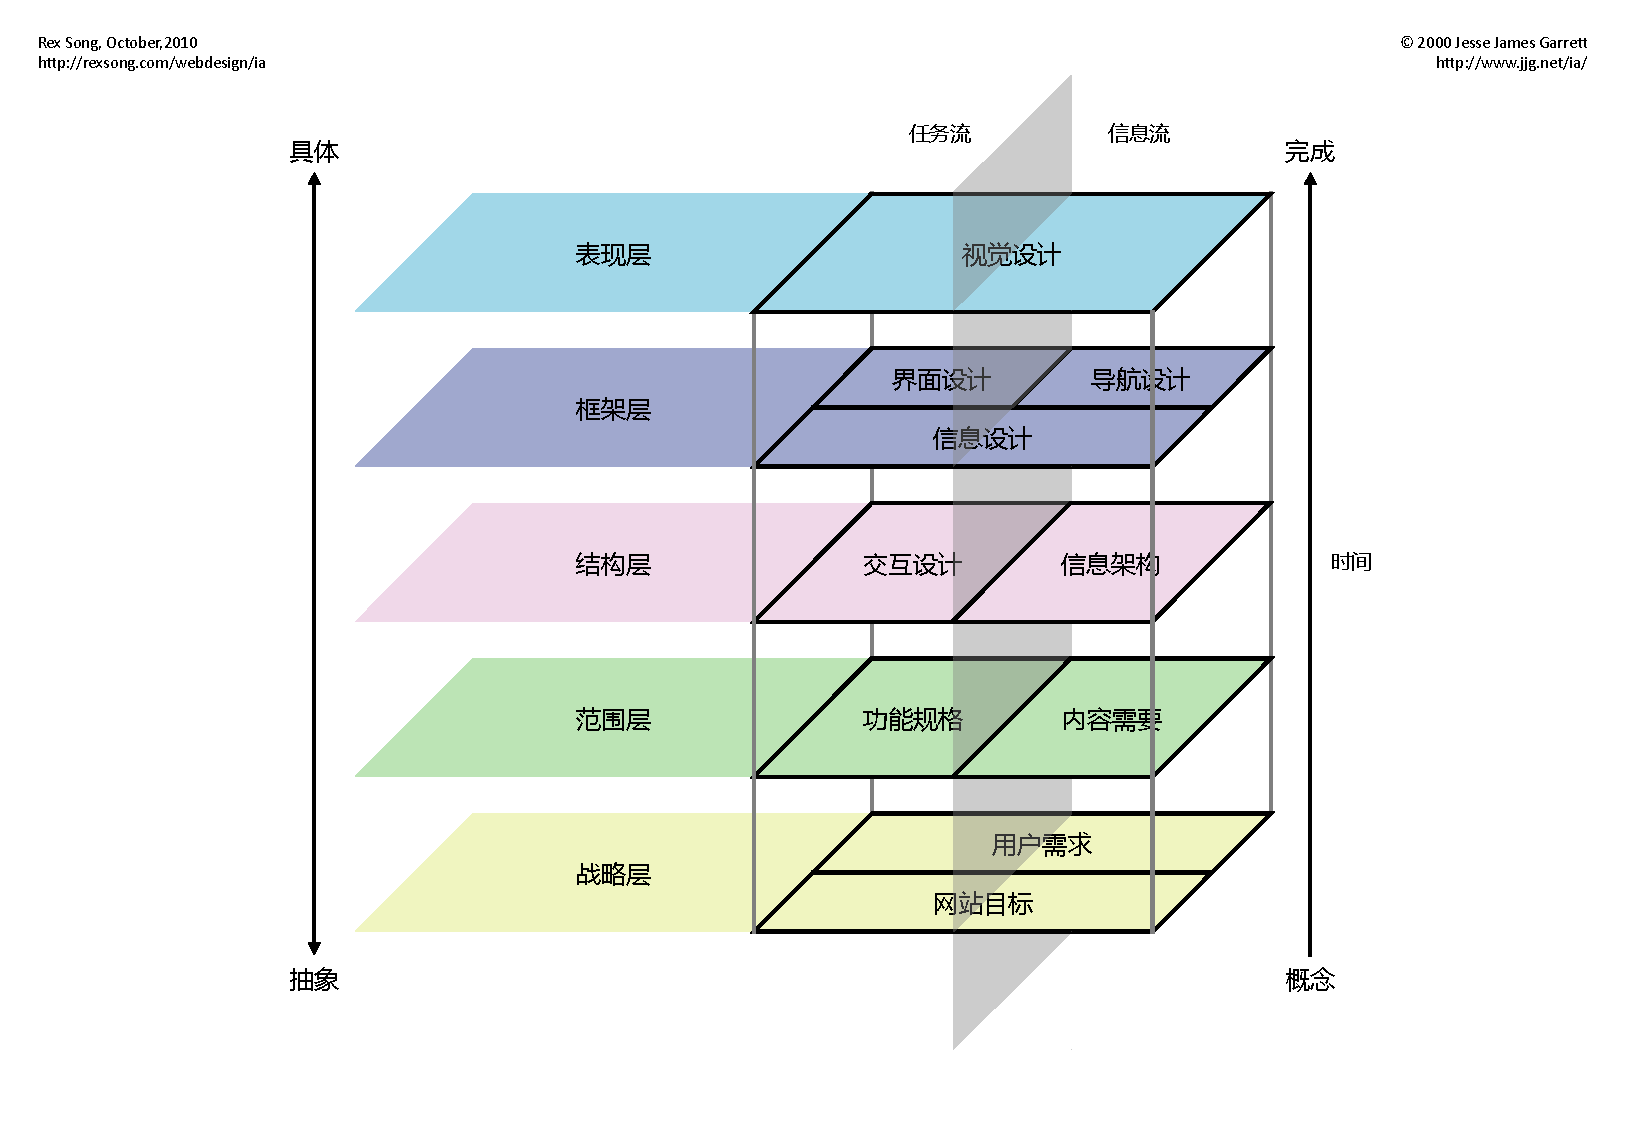
\includegraphics[scale=0.5]{model.pdf}\\
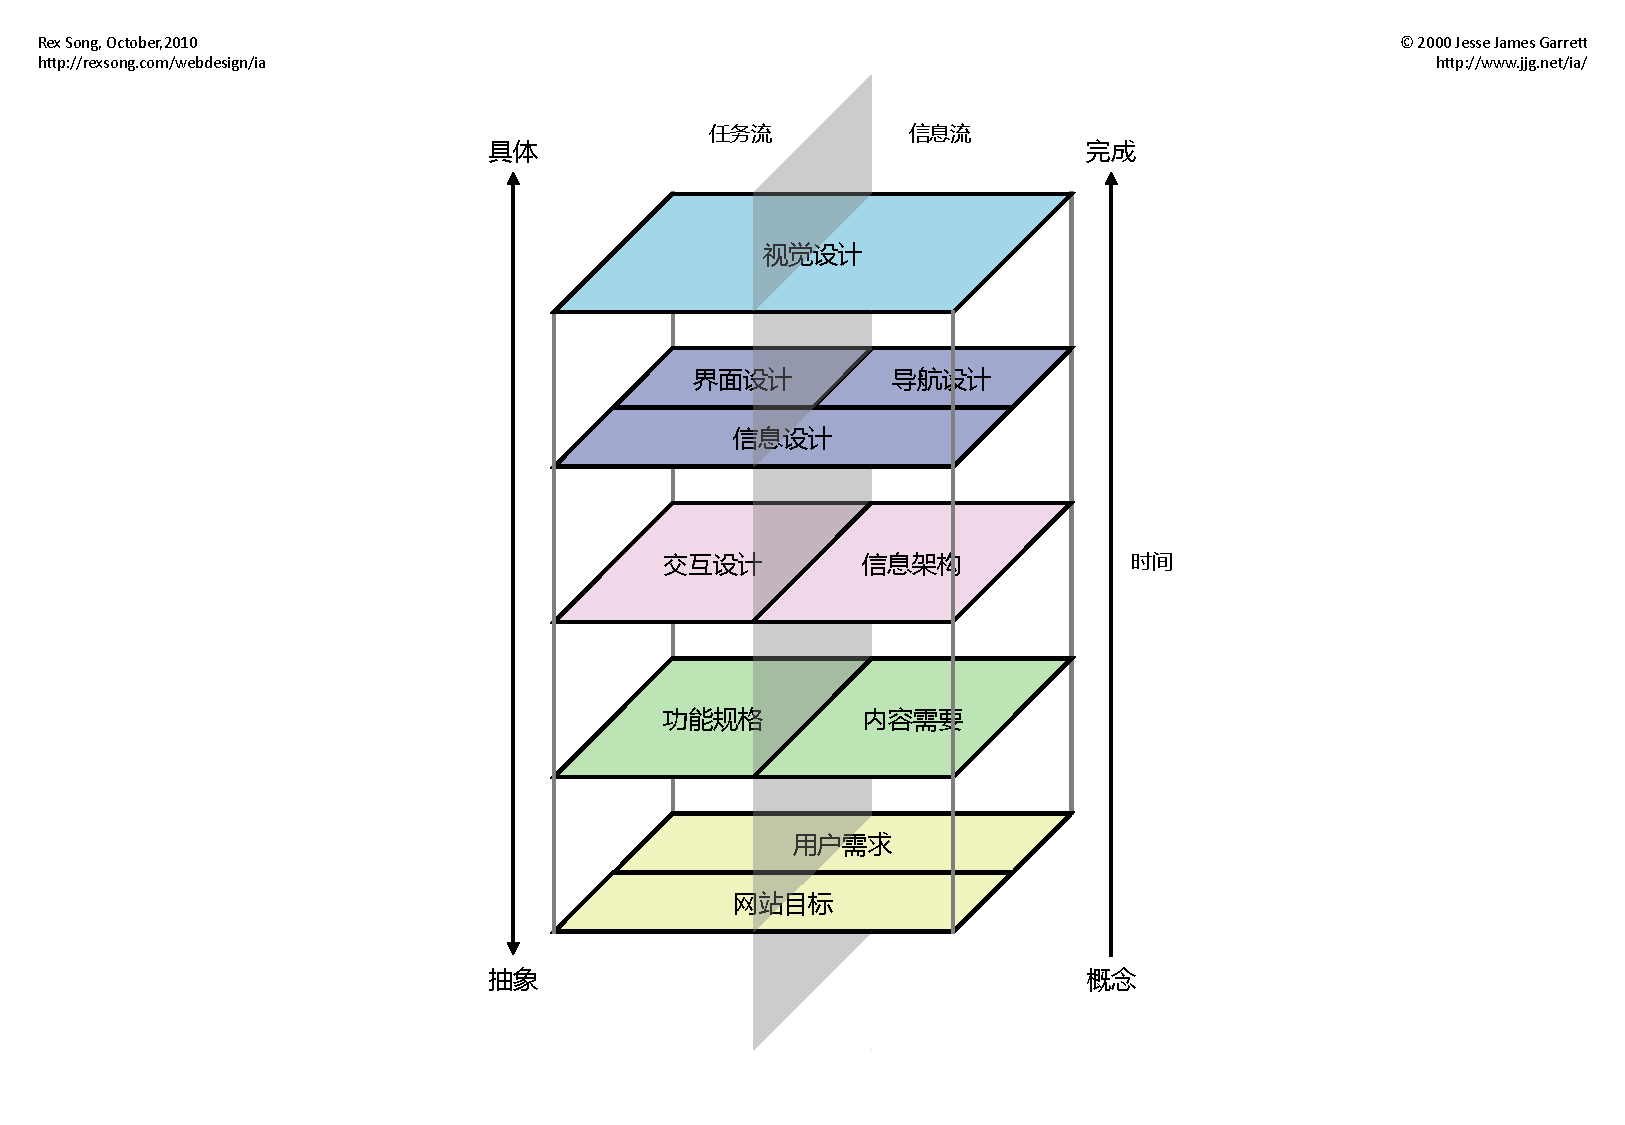
\includegraphics[scale=0.5]{models.pdf}
\end{figure}










\end{document}


























